%%% Local Variables:
%%% mode: latex
%%% TeX-master: t
%%% End:

\documentclass[bachelor,nofonts]{thuthesis}
%\documentclass[master]{thuthesis}
%\documentclass[doctor]{thuthesis}
% \documentclass[%
%   bachelor|master|doctor|postdoctor, % mandatory option
%   winfonts|nofonts|adobefonts, % mandatory only for bachelor and Linuxer
%   secret,
%   openany|openright,
%   arialtoc,arialtitle]{thuthesis}
% 当使用 XeLaTeX 编译时,本科生、Linux 用户需要加上 nofonts 选项;
% 当使用 PDFLaTeX 编译时,adobefonts 选项等效于 winfonts 选项(缺省选项)。

% 所有其它可能用到的包都统一放到这里了,可以根据自己的实际添加或者删除。
\usepackage{thutils}
\usepackage{listings}
\lstset{breaklines}

% 你可以在这里修改配置文件中的定义,导言区可以使用中文。
% \def\myname{薛瑞尼}

\begin{document}

% 定义所有的eps文件在 figures 子目录下
\graphicspath{{figures/}}


%%% 封面部分
\frontmatter

%%% Local Variables:
%%% mode: latex
%%% TeX-master: t
%%% End:
\secretlevel{绝密} \secretyear{2100}

\ctitle{脑健康测试系统研究}
\makeatletter
\ifthu@bachelor\relax\else
  \ifthu@doctor
    \cdegree{工学博士}
  \else
    \ifthu@master
      \cdegree{工学硕士}
    \fi
  \fi
\fi
\makeatother


\cdepartment[计算机]{计算机科学与技术系}
\cmajor{计算机科学与技术}
\cauthor{周若凡} 
\csupervisor{陶霖密教授}
% 日期自动生成,如果你要自己写就改这个cdate
%\cdate{\CJKdigits{\the\year}年\CJKnumber{\the\month}月}

\etitle{An Introduction to \LaTeX{} Thesis Template of Tsinghua University} 
% 这块比较复杂,需要分情况讨论:
% 1. 学术型硕士
%    \edegree:必须为Master of Arts或Master of Science(注意大小写)
%              “哲学、文学、历史学、法学、教育学、艺术学门类,公共管理学科
%               填写Master of Arts,其它填写Master of Science”
%    \emajor:“获得一级学科授权的学科填写一级学科名称,其它填写二级学科名称”
% 2. 专业型硕士
%    \edegree:“填写专业学位英文名称全称”
%    \emajor:“工程硕士填写工程领域,其它专业学位不填写此项”
% 3. 学术型博士
%    \edegree:Doctor of Philosophy(注意大小写)
%    \emajor:“获得一级学科授权的学科填写一级学科名称,其它填写二级学科名称”
% 4. 专业型博士
%    \edegree:“填写专业学位英文名称全称”
%    \emajor:不填写此项
\edegree{Doctor of Engineering} 
\emajor{Computer Science and Technology} 
\eauthor{Xue Ruini} 
\esupervisor{Professor Zheng Weimin} 
\eassosupervisor{Chen Wenguang} 
% 这个日期也会自动生成,你要改么?
% \edate{December, 2005}

% 定义中英文摘要和关键字
\begin{cabstract}
随着移动互联网不断的改朝换代,移动健康已经成为了医药产业信息化的一个重要的、必不可少的分支。认知功能障碍是痴呆的早期症状,如果得到及时的诊断并在临床上进行干预则可以很大程度上延缓病情的发展。传统的诊断基于纸质长问卷,费时费力。故依靠移动健康来辅助诊断认知功能障碍对于临床医学上具有非常重要的意义。

本文旨在基于安卓系统在移动平板上设计并开发一套能够辅助诊断认知功能障碍的医患交互系统,整个系统分成三个部分,包括在线病人版、在线医生版、离线打分版,目的在智能终端设备上能完全还原传统纸板的长问卷一样的体验,并将功能分开更易开发和使用;并实现多种题型如选择题、单词配对题、故事复述题等的界面,完成基于不同题目类型的数据记录、录音、笔迹记录等等;同时针对题目和系统对数据进行统一的设计,使测试得到的数据能比较好的整理,并且保证了系统的复用性和扩展性。
\end{cabstract}

\ckeywords{安卓,移动应用,人机交互,移动健康,脑健康}

\begin{eabstract} 
As the rapid development of mobile web, Mhealth has become an important and indispensable branch of informatization of medical industry. Cognitive dysfunction is the ealrly symptom of senile dementia, if cognitive dysfunction is diagnosed promptly, clinical intervention can largely postpone the development of the illness. While traditional diagnosis is based on long paper questionnaire which cost doctors' large time and energy. So it is with great significance using Mhealth to assist doctor to diagnose cognitive dysfunction.

This paper aims at design and develop a doctor-patient interaction system on panel computer to help docutor to diagnose cognitive dysfunction based on android. The whole system consists of three parts: patient-online version, doctor-online version and offline version, and it can totally restore the traditional long paper questionnaire on the mobile terminal devices and as well as being more easily for developing and using. And various types of questions is implemented such as choice question, learning trails question, story recall question and so on. Functions like data recording, audio recording, drawing recording is also implemented. The data system is also designed with the whole system so that the data could be well organized in the database, enable the system to have expansibility and reusability.
\end{eabstract}

\ekeywords{android, mobile application, human-computer iteraction, mHealth, brain-health}

% 设置 PDF 文档的作者、主题等属性
\makeatletter
\thu@setup@pdfinfo
\makeatother
\makecover

% 目录
\tableofcontents

% 符号对照表
%\begin{denotation}

\item[HPC] 高性能计算 (High Performance Computing)
\item[cluster] 集群
\item[Itanium] 安腾
\item[SMP] 对称多处理
\item[API] 应用程序编程接口
\item[PI]	聚酰亚胺
\item[MPI]	聚酰亚胺模型化合物,N-苯基邻苯酰亚胺
\item[PBI]	聚苯并咪唑
\item[MPBI]	聚苯并咪唑模型化合物,N-苯基苯并咪唑
\item[PY]	聚吡咙
\item[PMDA-BDA]	均苯四酸二酐与联苯四胺合成的聚吡咙薄膜
\item[$\Delta G$]  	活化自由能~(Activation Free Energy)
\item [$\chi$] 传输系数~(Transmission Coefficient)
\item[$E$] 能量
\item[$m$] 质量
\item[$c$] 光速
\item[$P$] 概率
\item[$T$] 时间
\item[$v$] 速度
\item[劝  学] 君子曰:学不可以已。青,取之于蓝,而青于蓝;冰,水为之,而寒于水。
  木直中绳。(车柔)以为轮,其曲中规。虽有槁暴,不复挺者,(车柔)使之然也。故木
  受绳则直, 金就砺则利,君子博学而日参省乎己,则知明而行无过矣。吾尝终日而思
  矣,  不如须臾之所学也;吾尝(足齐)而望矣,不如登高之博见也。登高而招,臂非加
  长也,  而见者远;  顺风而呼,  声非加疾也,而闻者彰。假舆马者,非利足也,而致
  千里;假舟楫者,非能水也,而绝江河,  君子生非异也,善假于物也。积土成山,风雨
  兴焉;积水成渊,蛟龙生焉;积善成德,而神明自得,圣心备焉。故不积跬步,无以至千
  里;不积小流,无以成江海。骐骥一跃,不能十步;驽马十驾,功在不舍。锲而舍之,朽
  木不折;  锲而不舍,金石可镂。蚓无爪牙之利,筋骨之强,上食埃土,下饮黄泉,用心
  一也。蟹六跪而二螯,非蛇鳝之穴无可寄托者,用心躁也。\pozhehao{} 荀况
\end{denotation}



%%% 正文部分
\mainmatter

%%% Local Variables:
%%% mode: latex
%%% TeX-master: t
%%% End:

\chapter{引言}
\label{cha:intro}

\section{研究背景}

认知功能障碍指的是记忆障碍和轻度的其他认知功能障碍,是痴呆的早期症状,重要的临床意义在于早期发现和早期干预,可以延迟甚至阻止痴呆的发展。\footnote{摘自中华老年医学杂志2006年7月第25卷第7期 《中国防治认知功能障碍专拣共识》}然而由于认知功能障碍表现形式非常多样化,在不同个体上体现的如记忆力快速下降、时间能力受损、计算能力障碍、空间定向障碍、语言理解执行能力下降、判断力下降、逻辑判断能力障碍等等,诊断需要对被试人各个方面(记忆,逻辑,计算,语言,绘画等等)均进行测试,故传统的诊断方式为使用医疗问卷进行医患一对一的评估。医疗问卷涵盖了上述各个方面的测试,测试内容包括故事复述题、重复数字题、逻辑选择题、记忆绘画题、回忆绘画题等等,问卷长达103页,医生使用手册长达131页,要学习如何正确打分需要至少一年的训练和学习。在测试过程中医生除了需要在纸上勾选、记录病人的回答,也需要用音频记录病人的一些回答,有一些题目也需要病人在纸上进行绘画,测试中还需要医生通过一些现场观察进行一些问卷之外的诊断,这些纸质和媒体记录的方式虽然为诊断提供了大量的信息,也使得数据量不断庞大,这些基于不同媒体介质的数据使得后期病例整理非常麻烦。

信息技术的发展使得移动健康变成了医药产业的一个重要的分支,医疗服务信息化也已经成为了国际趋势,越来越多的国内外医院开始引进信息技术来辅助一些医疗服务\footnote{引自“Design and implementation of doctor-patient interaction system based on android”}。北京协和医院和波士顿大学与清华大学寻求合作,希望共同开发脑健康评估系统,目的在能基于安卓系统开发一套医患交互系统,能够利用移动互联网的优势辅助认知功能障碍的诊断,并能在平板电脑上完全还原传统纸板的系统,能够系统地组织整理测试所得数据(文字答案,语音和绘画轨迹),同时也界面设计也希望能够方便易懂、使医生能够在段时间内学会如何使用系统。

\section{研究现状}

美国、日本以及一些欧洲国家非常重视相关疾病的研究,美国建立了近30个专业研究中心,每年的研究经费超过10亿美元,欧洲国家在这个领域上投入也超过1亿欧元。经过十多年的临床实验和数据分析,国际上有一些公认的简易诊断工具,如Mini-Cog,MMSE,MoCA,GPCOG等等,这些工具需要测试患者的认知功能的各个方案,但这些工具只能提供辅助性的判断,如需确诊还需要进一步更深入的测试。波士顿大学向我们提供的《神经心理学测试长问卷》\footnote{原名:“Neuropsychological Test Battery”}就是这样一个“更深入”的测试问卷,这个长达103页的测试包括多种题型,全面测试患者的记忆、逻辑、计算、语言、绘画等认知功能的多方面功能,通过这些测试结果综合评分,可以确定测试患者是否已患认知功能障碍。

虽然该疾病领域的研究已经发展了十多年,但仍然停留在传统的纸质长问卷上,目前还没有一个自动诊断系统,“目前所有应用于医学测试的系统都只是文字版的”\footnote{引自“Systems and methods for the physiological assessment of brain health and the remote quality control of EGG systems”}。

\section{设计内容}

本文提出了一个基于android系统、建于平板电脑的脑健康评估系统。本系统为配合医生进行认知性功能障碍诊断使用,设计并实现了多种题型包括选择题、轨迹记录题、故事复述题、单词对记忆题、数字串复述题、图片展示题等展示和使用的界面,并包含了数据记录、音频录制、轨迹记录等多个功能。为后期数据方便整理,对题目格式、数据格式针对系统进行了统一的规划和设计,并对数据的存储位置进行了考量和设计。在界面中加入了防错和引导功能,使医生能够在段时间迅速学会使用这个系统进行诊断。

\section{论文的组织结构}

本文第一张详细描述了本系统设计和开发的背景,主要介绍了国内为认知功能障碍的诊断方法现状,讨论了设计和开发本系统的重要意义。

第二章介绍了本次开发使用的平台、工具和问卷资料。

第三章根据问卷资料和医院的需求进行了需求分析,并根据需求对整个系统和数据存储进行了框架设计。

第四章根据系统需要的语音识别功能进行了相关实验并提出了使用百度云语音识别的结论。

第五章根据框架设计,针对每一个模块进行了细节分析、设计和实现。

第六章介绍了对系统的测试。

第七章对本系统设计的实现进行了总结。



%%% Local Variables: 
%%% mode: latex
%%% TeX-master: t
%%% End: 

\chapter{问卷、平台和工具}

本系统设计基于波士顿大学提供的《神经心理学测试长问卷》及其使用说明文档,通过安卓平台进行了设计,硬件设备选择了联想的YOGA Pro2平板,通过实验选择使用了百度语音开放平台的API接口实行语音识别功能,并选择使用阿里云的开放存储服务OSS作为数据存储位置。本章节就这些资料、平台和工具做简要的介绍,并讨论选择使用的原因。

\section{《神经心理学测试长问卷》介绍}

《神经心理学测试长问卷》已经运用超过了十年\footnote{引自“10 Years of the Neuropsychological Test Battery”}。经过数年来的实验和资料的累积,这份问卷也不断更新,除了传统的一些关于记忆力、习题、语言等测试,也加入了绘画、计算等题目。由于其题目的特殊性(需要有人引导和控制,并对病人进行观察),所以一直沿用传统的“纸笔测试”。通过对该测试各项进行综合打分,可以对病人是否患有认知功能障碍进行精准的判断。然而,由于包括的题目类型和数量繁多、结构比较复杂、操作难以学习,虽然该问卷也有建议版本,但整个问卷的完成依旧需要至少4个小时,而实施的医生也至少经过一年的学习和观察才可以真正上岗对病人进行测试。

\begin{table}[htbp]
\centering
\caption{问卷的题目类型说明表(部分)}
\label{tab:ParametersForPandR}
\begin{tabular}[c]{lcccc}
\toprule[1.5pt]
{\heiti 测试类型} & {\heiti 领域} & {\heiti 第一次测试类型} & {\heiti 第二次测试类型}\\\midrule[1pt]
视觉配对 & 记忆力 & 立即复述 & 延时复述\\
语言配对 & 记忆力 & 立即复述 & 延时复述\\
语言学习测试 & 记忆力 & 立即复述 & 延时复述\\
控制口语测试 & 执行力 & 可认可单词数 & -\\
流利分类测试 & 执行力 & 可认可单词数 & -\\
数字串重复测试 & 执行力 & 正确复述的数字串长度 & -\\
\bottomrule[1.5pt]
\end{tabular}
\end{table}

虽然整个问卷系统需要电子信息化,但为了和十多年的实验和研究资料进行匹配和兼容,对设计到平板电脑上的系统需要几乎完全还原纸板系统上的体验,才能保证在这样系统辅助的测试环境与传统纸笔测试的环境相同,才能够保证测试结果和之前统计的结果相对应。

\section{Android平台介绍}

\subsection{Android介绍}

Android(安卓)是基于Linux内核的一款给移动设备设计的操作系统,目前由Google公司进行开发。为了能够通过屏幕直接操作,Android的设计主要是为了触摸屏移动设备(如智能手机或平板电脑),也可以用于一些特定的电视、车辆或穿戴设备(手表等)。用户可以在触摸屏上进行多种触摸操作,如点击,拖动,滑动等等,它也为用户提供虚拟键盘用于一些文字的输入。\footnote{本段部分内容翻译自Android的维基百科主页http://en.wikipedia.org/wiki/Android\_(operating\_system)}。

Android是开源的系统,便于、也吸引了很多开发者在系统上进行更新或开发。目前Android系统已经开发特别成熟,除了精美的界面,还提供非常多的服务,例如WIFI、拍照、录音、文件存储、蓝牙、GPS定位等等,这些服务都可以便于我们对脑健康系统的开发。另外对比IOS系统,Android上开发应用完全免费,且拥有多个便捷的开发工具。Google为Android开发提供了详尽的软件开发工具(称作SDK),包括了调试器、软件库、一系列模拟器,也包含了一些样例代码和入门文档。其提供的软件库包含了很多调用Android服务的接口,例如界面组件、媒体播放器、文件存储读取等等,故在安卓平台上开发一个系统(一个应用APP)是相对容易、便捷的。

\begin{figure}[h]
  \centering
  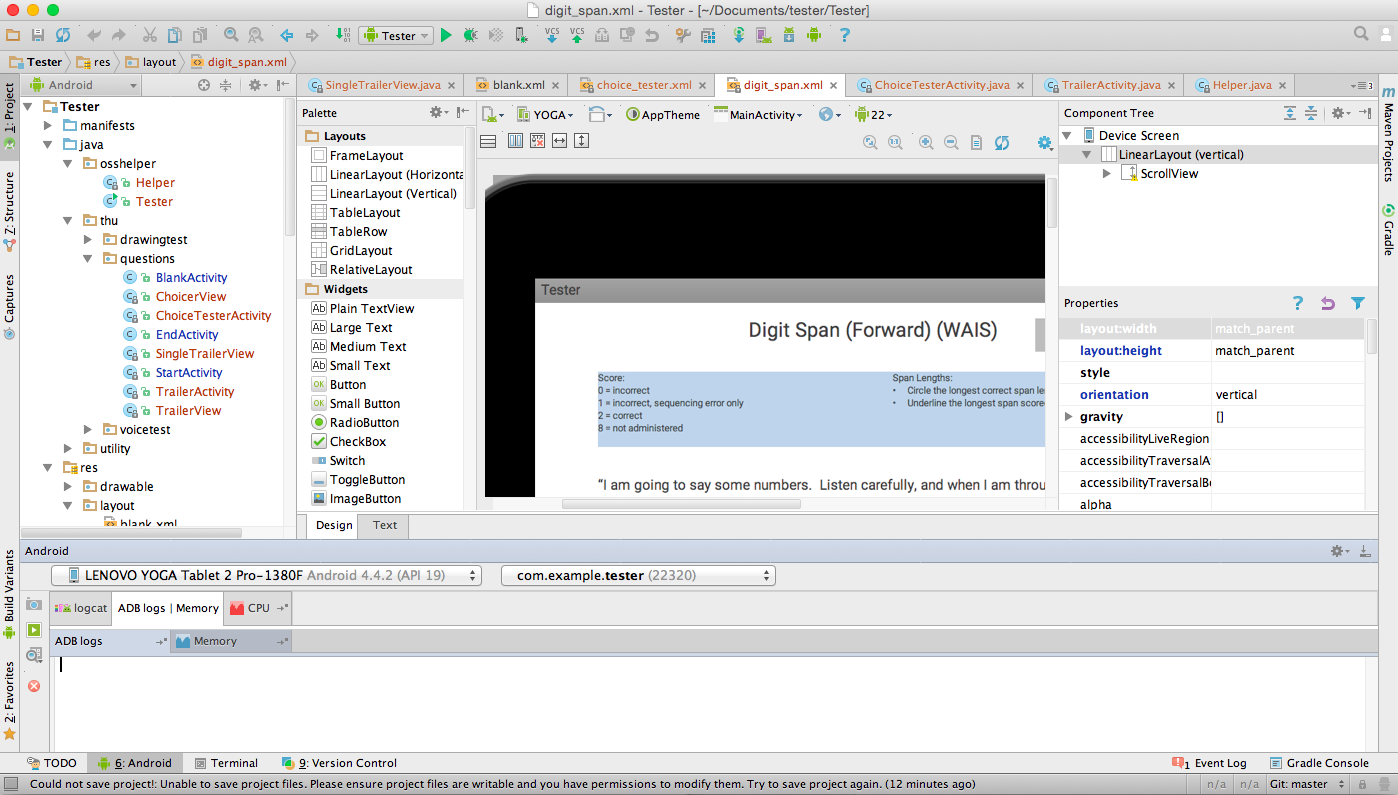
\includegraphics[width=13cm]{chapter1-1}
  \caption{AndroidStudio使用界面}
\end{figure}

\subsection{Android Studio平台介绍}

本次开发Android应用选用了Android Studio这个IDE,它由Google于2013年5月发布,该IDE针对安卓开发,融合了SDK和ADT的版本检查和安装,方便地控制编译的版本;拥有便捷的可视化布局,可以实时编码、实时程序界面浏览;拥有可以协助翻译、优化提示、来源跟踪的开发者控制台,让开发者更舒适地进行编码;基于Gradle地构建支持,也可以方便地和Eclipse开发的Android工程进行相互转化;拥有Android特定的代码重构和快速修复;拥有能对程序性能、可用性、版本兼容等各种问题进行控制捕捉的提示工具;支持应用签名;自带方便的布局编辑器,可以让开发者拖动UI组件,也可以预览在不同设备(可自定义)上UI的显示效果。总体来说,AndroidStudio是一款比Eclipse更便捷、更全面,而又更轻量的的Android开发平台。

\section{联想YOGA平板介绍}

本次系统设计选用的平板电脑为YOGA Pro-1380F,除了拥有其他平板电脑的特点,它拥有13.3英寸的大屏和2560*1440分辨率。基于Android4.4系统深度优化,可以运行所开发的系统。

为了满足“和纸笔测试保持一致”的要求,应用平台应该满足可以记录绘画内容、屏幕大小和标准A4纸相差不打的要求,YOGA Pro-1380F均满足了这些需求。

\begin{figure}[h]
  \centering
  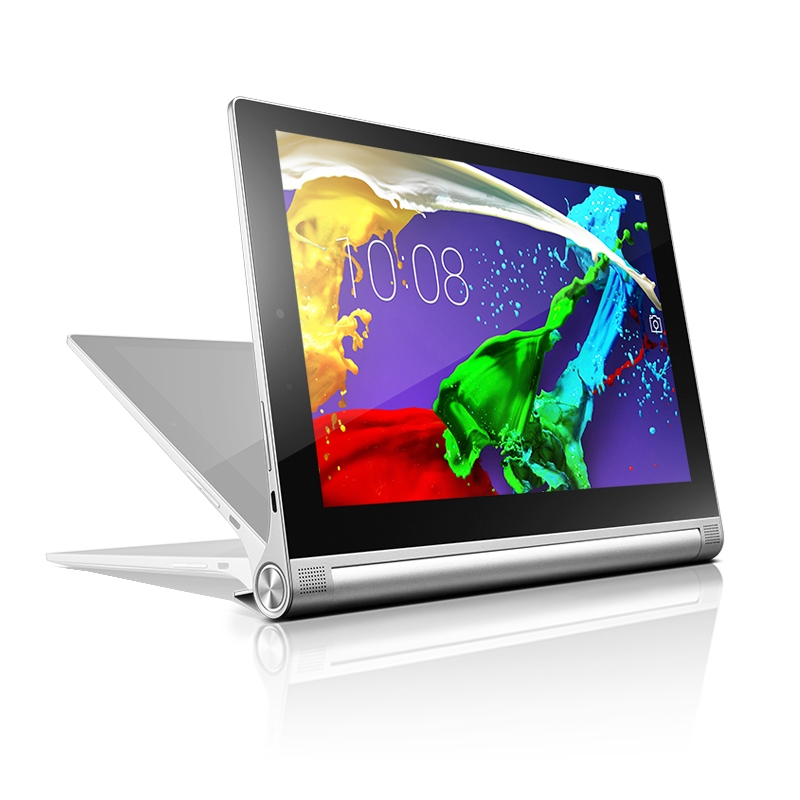
\includegraphics[width=13cm]{chapter1-2}
  \caption{YOGA Pro-1380F}
\end{figure}

\section{阿里云开放存储服务介绍}

阿里云开放存储服务(Open Storage Service,简称OSS)是阿里云对外提供的云存储服务,具有海量、安全、可靠性高的特点。其稳定,系统规模能够在不影响对外服务的前提下自动扩展,数据会进行三重备份,并可以设置日志记录,可靠、丢失易找回;系统通过多层次安全防护,也设置了防DDoS攻击,设有多用户隔离机制,也可以通过日志记录来追查非法访问;为背景用户提供了免费的5GB存储空间,还可以无限量扩展,请求处理能力会根据压力弹性增加,设置了多线BGP网络确保全国各地甚至国外都能访问流畅。另外,阿里云开放存储服务还提供了图片处理的工具,能够对存储在OSS上的图片进行缩略、压缩、裁减、水印和格式转换等图片处理功能。平台提供了详尽了开发者资源(兼容Python,Java,.NET,PHP,iOS,Android,NodeJs)、操作手册和第三方工具,使得基于此平台的开发和数据管理都相当方便。另外官方提供了100倍故障赔偿和全天24小时的售后支持,诸多有名的互联网产品都在此平台上搭建了自己的数据库,如微盟、筋斗云呼叫系统、得图云等等。

本系统的设计所需要的数据类型主要是文字(一些选择选项或是答案)和流媒体(图片,音频或视频),每次测试所生成的数据不超过5MB,故OSS平台提供的5GB的免费空间完全足够开发这个系统测试所需。另外OSS平台的日志记录等特点也适合在开发过程中进行调试;平台提供的Android SDK也为开发提供了便捷的接口,也无需担心服务器地址的移动,同时也利用平台安全、可靠的特性保证了数据的隐密性。故OSS平台是相当适合做该系统数据存储的平台的。

\section{百度语音开放平台介绍}

百度语音开放平台提供了免费的完全永久免费的语音识别服务,不仅支持多种语言(中文、英语、粤语),还提供了基于35个领域的语义解析,依托了百度多个服务(知道、贴吧等社区产品)上累积的强大知识库,能够做到智能推理,提高识别性能。使用场景包括语音搜索、语音输入、语音转写、语音助手等。

本系统的设计在一些语音题上需要运用语音识别系统进行识别,目的在于减少用户对相关文字的输入。通过一系列对目前市场上开放的语音识别服务的评测和实验(后续章节会详细说明),最终选择了百度语音开放平台。




%%% Local Variables: 
%%% mode: latex
%%% TeX-master: t
%%% End: 

\chapter{需求分析与系统框架设计}

\section{业务需求分析}

如今,走向科学化、信息化,通过数据来分析才能更好的进行诊疗,当代医学的已经不能再仅仅依靠医生的经验通过望闻问切进行诊断。如之前所阐述,认知功能障碍表现多样而导致诊断需要针对患者的各项能力进行评测,并通过均衡各项的分数而得出结论。由于传统纸笔测试的繁琐、学习成本大、题量繁多,导致数据不易存储、诊断不方便、学习代价大等等困难。而开发这样一款电子问卷可以很好的解决这些问题,能够更好地组织所有的数据。同时,波士顿大学和北京协和医院都和我们提出了合作的请求,希望开发这样的方便的系统辅助医生进行诊断和数据整理。开发这样的脑健康评估系统是走在了中国乃至世界脑健康研究的前列,可以推动脑健康研究的发展,也可以巩固合作医院的业界地位。

\section{功能需求分析}

脑健康研究系统要求完成一个辅助医生诊断认知功能障碍的系统。系统包括多种题目包括信息录入、选择题、录音题、画图题。最终系统需要对用户录入的信息进行统计整理、并对做的题目进行评分(画图题只需针对流畅性给出辅助性的评分,语音题能够做一些适当的识别,其余需要根据评分标准给分),对认知功能障碍做一个初步的诊断。

\subsection{故事复述题}

\begin{figure}[h]
  \centering
  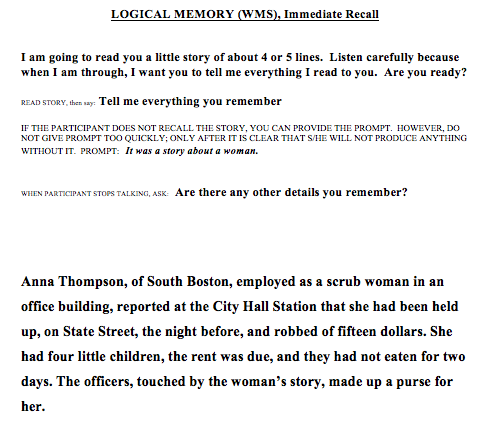
\includegraphics[width=13cm]{chapter2-1}
  \caption{原问卷中的故事复述题}
\end{figure}

故事复述题为医生为病人讲述一个4-5行的小故事,然后让病人立即复述这个故事的内容,医生可以给一些提示(如“这是一个关于女人的故事”)。变为电子问卷后需要拥有以下需求:

\begin{itemize}
\item 存储故事的录音、可以播放故事的录音。
\item	可以将病人全部的讲述的音频录制下来并保存、后期可以调出录音进行评分。
\item 与问卷一样拥有提示语句。
\end{itemize}

另外希望能够为该类型的题目提供辅助打分功能:

\begin{itemize}
\item 播放测试时录制的病人陈述。
\item	对录音进行语音识别。
\item	与打分问卷一样的打分版面。
\end{itemize}

\subsection{图片复原题}

\begin{figure}[h]
  \centering
  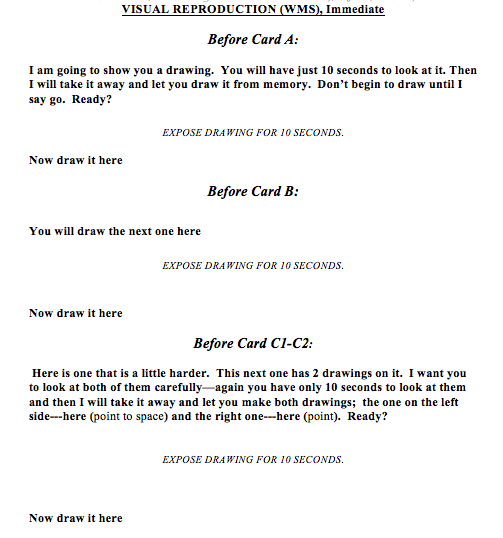
\includegraphics[width=13cm]{chapter2-2}
  \caption{原问卷中的图片复原题}
\end{figure}

图片复原题为医生会给病人依次展示三张图片卡片(每个展示十秒),结束后记录病人绘画的轨迹。变为电子问卷后需要拥有以下需求:

\begin{itemize}
\item 可以存储需要展示的图片、并能控制其显示十秒钟后消失。在图片展示时,提示语句不应该出现。
\item	能记录病人绘画的轨迹过程。在绘画后面的图片时,前面的图片应该还在其视野中。
\item 与问卷一样拥有提示语句。
\end{itemize}

另外希望能够为该类型的题目提供辅助打分功能:

\begin{itemize}
\item 展示病人之前绘画的轨迹。
\item	与打分问卷一样的打分版面。
\end{itemize}

\subsection{单词配对题}

\begin{figure}[h]
  \centering
  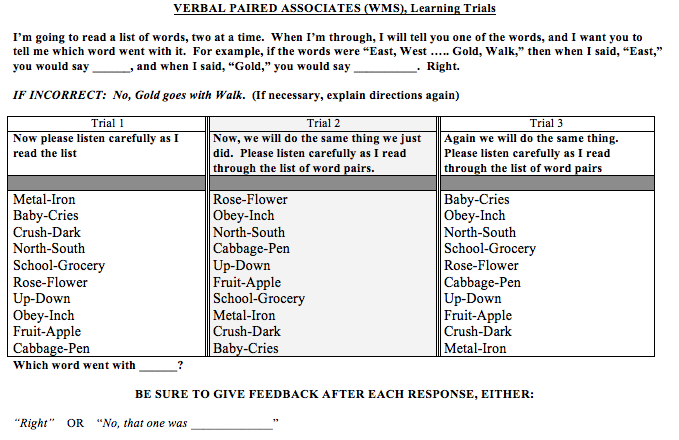
\includegraphics[width=13cm]{chapter2-3}
  \caption{原问卷中的单词配对题}
\end{figure}

单词配对题为医生会为病人读连续十个单词对,之后向病人进行提问,根据病人回答的单词进行评分(分为正确、有关错误、无关错误、搞混错误)。变为电子问卷后需要拥有以下需求:

\begin{itemize}
\item 可以存储读单词对的录音并进行播放。
\item	界面能便于医生进行答案记录和打分。
\item	需要记录错误答案的类型(以字典形式)。
\item	能够根据选择计算总得分。
\end{itemize}

\subsection{延期复述题}

\begin{figure}[h]
  \centering
  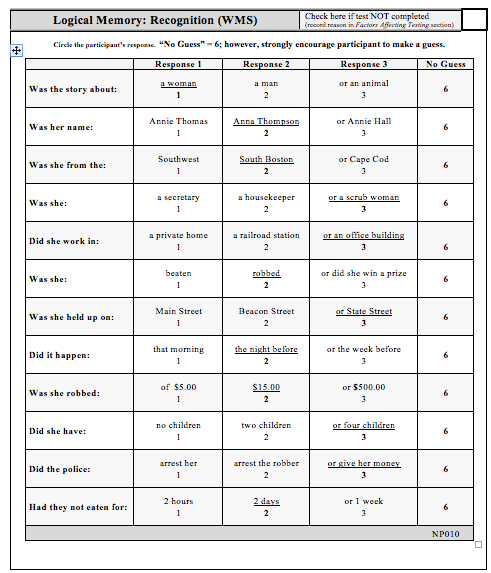
\includegraphics[width=13cm]{chapter2-5}
  \caption{原问卷中有关故事复述的延期复述题}
\end{figure}

很多类型的题目都拥有延期复述题(如故事复述题、图片复原题、单词配对题都有),是在这些题目测试结束之后一段时间再进行测试,主要考察病人的长期记忆力。该题目主要是选择题(但也有其他题目类型)。变为电子问卷后需要拥有以下需求:

\begin{itemize}
\item 可以展现题目、并能让医生方便的看出正确答案。
\item	能够方便的记录病人的回答,也能对病人的答案进行“一键式”评分。
\end{itemize}

\subsection{数字串复述题}

\begin{figure}[h]
  \centering
  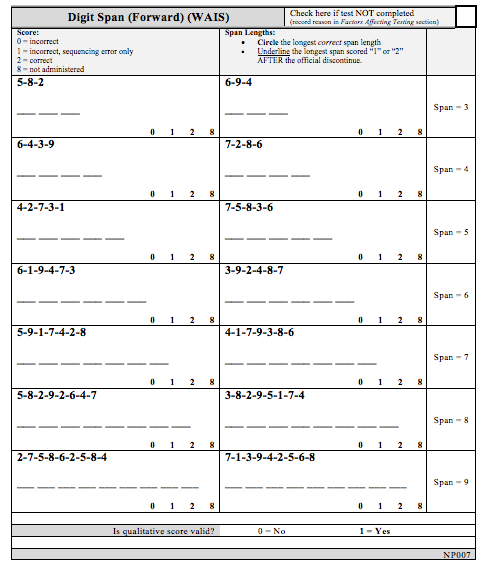
\includegraphics[width=13cm]{chapter2-4}
  \caption{原问卷中的数字串复述题}
\end{figure}

数字串复述题分为两类,一类为“顺序”,另一类为“逆序”。顺序数字串复述题为医生为病人说一串数字,病人需要按照顺序复述;逆序数字串复述题则需要病人按照逆序复述,逆序数字串复述题还拥有引导病人的两道题目。如果病人数字和顺序都正确,则可以获得两分,如果只有数字是正确的,则可以获得1分,否则只有0分。该题目最终得分为两个数值,一个是最长正确复述数字串长度,另一个是无关顺序最长正确复述数字串长度,每个长度的数字串有两道题目,如果都得了0分则测试结束。变为电子问卷后需要拥有以下需求:

\begin{itemize}
\item 展现题目、能够方便记录病人答案,也能让医生方便的看到正确答案。
\item	能够计算两个分值:最长正确复述数字串长度和无关顺序最长正确复述数字串长度。
\item 能够对医生做一定引导,告诉医生下一个测试的数字串是什么。
\end{itemize}

\subsection{其他需求分析}

其他需求包括界面的要求、网络的要求等等,主要归纳如下。

\begin{itemize}
\item 需要与纸板问卷有一样的体验,展示界面应该和标准A4纸大小类似。
\item	界面应该尽量还原原来问卷的界面,并且对使用者有一定引导性、方便好用。
\item 能有效组织题目和病人数据。
\item 界面友好。
\end{itemize}

\section{系统框架设计}

\begin{figure}[h]
  \centering
  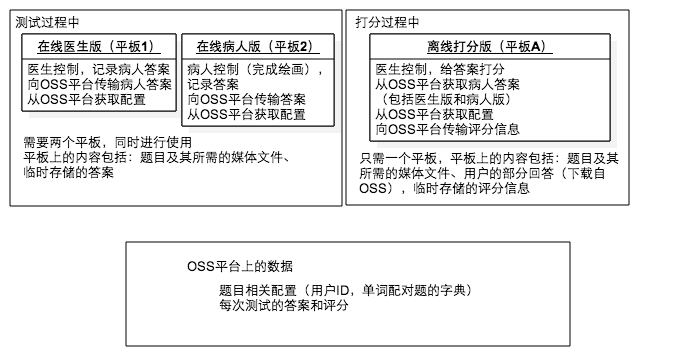
\includegraphics[width=13cm]{struct}
  \caption{三个版本的关系说明图示}
\end{figure}

根据上述需求,最终设计的系统分成三个版本:在线医生版、在线病人版和离线打分版,并用JSON格式化了整个系统的数据(包括题目的存储和病人的回答),以及用Java面向对象的继承特性设计大体框架和底层逻辑。

\subsection{三个版本}

为了满足和纸板问卷一样的体验的要求,并且保证开发过程中的便捷,整个系统分成三个独立的版本,两个在线版本用来复原原问卷的测试部分,而离线版本可以对测试得到的结果进行一定的评分和修正。这三个版本虽然没有相互的通讯,但是共享一个数据库(题目和测试结果),保持了开发的简单性和数据的统一性。

\subsubsection{在线医生版}

在线医生版为医生在测试时使用的,涵盖了原问卷大部分的题目(如故事复述题)。该版本不仅需要还原原问卷上的这些题目,也需要给医生提供一些引导语句和引导图示,同时也需要针对操作失误进行防范。

\subsubsection{在线病人版}

在线病人版为病人在测试时使用的,主要为了满足原问卷中一些医生和病人都需要纸板问卷的题目(如图片复原题)。不合并在线医生版和病人版的原因是这样不仅可以和原问卷这些题目一样双方都拥有问卷的体验,同样也将一些题目拆分开,使开发过程中一类题目不用分成两种不同的实现版本,更加简化了设计和开发。

\subsubsection{离线打分版}

离线打分版用于在测试过后医生重新调出之前测试的结果并进行打分,在这个版本中不仅需要给出人工评分、勾选的功能,也需要设计一些自动算法进行辅助性评分(如进行语音识别、轨迹识别等)。

\begin{figure}[h]
  \centering
  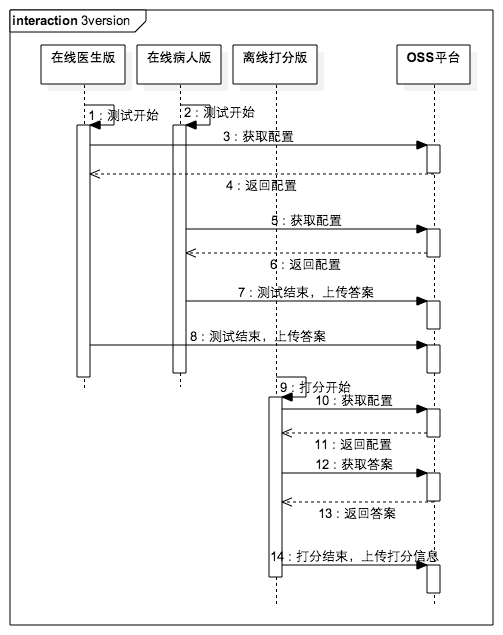
\includegraphics[width=13cm]{3version}
  \caption{一次测试中三个版本的使用说明图}
\end{figure}

\subsubsection{三个版本的关系说明}

在测试时,分别使用两个平板作为使用在线医生版和在线病人版的媒介并分别给予病人和医生使用。平板上存储有关题目的所有信息(包括媒体文件),但是需要从OSS平台上下载配置(因为题目的不变性和配置需要改变的特性)。在测试结束后要向OSS平台上传该测试得到的答案。

在打分时,只需要一个平板(可以复用在测试时使用的在线医生版)用于医生使用。平板上存储有关题目的所有信息,同在线版本一样需要从OSS平台上下载配置,也需要在OSS平台上下载用户的相关答案。在打分结束后需要向OSS平台上传打分的信息。

\subsection{数据系统设计}

在这次系统设计中,题目有关的数据存在了APP内部(Android工程的res文件下),包括题目的文字、画图题的图片、音频题需要播放的录音,这样保证在APP上题目可以瞬间读出而不需要再从网络上获取,因为题目已经固定无需修改,固定在APP中使得这些数据不会遭到操作失误而导致的修改,也使得逻辑部分的实现变得简单。而病人的测试数据和结果、以及APP的一些配置文件放在阿里云的开放存储平台上,这样可以使三个版本都能方便的读取、修改和评分。其中题目的文字和病人的一些可以用文字表达的答案均使用了JSON格式化。

这样的数据系统具有性能快、开放、安全、可靠、可操作性强等特点。

\subsubsection{JSON格式介绍}

JSON(全程JaveScript Object Notation)是一个轻量级的数据交换语言,以文字为基础,且易于让人阅读,现在已经成为一个独立于语言的文本格式。JSON用于描述数据结构,有以下形式存在:

\begin{itemize}
\item 对象:一个对象以左花括号开始,用右花括号结束。一个对象包含一些列并序列的名称-值对,每个名称-值对之间使用逗号分割。
\item 名称-值:名称和值之间使用冒号分割,一般形式为:
\begin{lstlisting}[language=JAVA]
{name:value}
\end{lstlisting}
其中名称一定是一个字符串(用双引号扩起来的一串字符),一个值可以是一个字符串,可以是一个数值(一系列0-9的数组组合,也可以是负数或小数,也支持用e或E表示指数形式),可以是一个布尔值(true或false),可以是一个对象,可以是一个有序列表,也可以是一个空值(null)。
\item 值的有序列表:一个或者多个值用逗号分区后,使用左大括号和右大括号括起来的一个列表,如:
\begin{lstlisting}[language=JAVA]
[collection, collection]
\end{lstlisting}
\end{itemize}

JSON由于其便捷、易懂、表达能力强的特性应用范围广泛。在数据系统的设计中使用JSON是因为可以方便的利用它定义任何文字表达的数据,且在Java的内部库中已经包含了对JSON格式读取、存储的API,使利用JSON开发数据系统的代价非常小。

\subsubsection{题目资源数据}

这部分由于数据的固定性,也为了开发的方便,直接固定在了APP内部,均存放在Android工程的res文件下。其中题目用JSON格式化,这样便于不同题目类型可以统一地存放在一个文件中,也方便后续对新题型进行扩展,同时也容易修改或者增加其他新的特征(原题目和JSON格式化后的示例可以见图3.8)。

\begin{figure}[h]
\centering%
\begin{subfigure}{13cm}
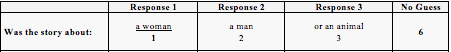
\includegraphics[width=13cm]{JSON_OQ}
\caption{原问卷中的题目}
\end{subfigure}
%\hspace{4em}%
\begin{subfigure}{6cm}
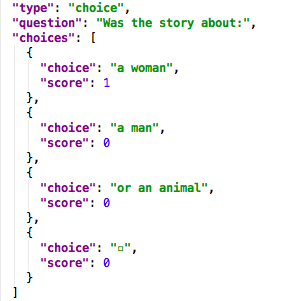
\includegraphics[width=6cm]{JSON_Q}
\caption{JSON格式化的题目}
\end{subfigure}
\hspace{4em}%
\begin{subfigure}{6cm}
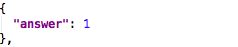
\includegraphics[width=6cm]{JSON_A}
\caption{JSON格式化的示例答案}
\end{subfigure}
\caption{题目和对应题目JSON、答案JSON示例}
\label{fig:big1-subfigure}
\end{figure}

JSON格式化后的题目主要包含以下几个名称-值对:

\begin{itemize}
\item type(类型):表示当前题目的类型,有choice(选择题)、story\_recall(故事复述题)、digit\_span(数字串复述题)、trailer(单词配对题)、draw(图片复原题)等。
\item guide\_word(引导词):表示该题目的引导词。
\item record(记录名):说明该题目需要进行音频录制,此值表示的是需要上传录音文件的名字。
\item skip(跳过):表示如果该题目被跳过,则这个值中的题目序号也需要被跳过。
\item down(下标):表示界面上右下角该题目应该显示的标号。
\end{itemize}

还有需要针对不同题目设计的不同名称-值对来完整的表达这道题目。

\subsubsection{配置数据和答案数据}

由于这部分的数据可能需要进行修改,且答案数据需要具有隐密性,所以选择将这些数据存储在了阿里云的开放存储平台上,这个平台上的能保证这些数据的安全性、隐私性,也给了一定备份方案,使数据不易丢失。为了后期数据的管理,这些数据有组织地存储在平台上,结构可见图3.9。其中配置文件(包括医生-患者对、trailer所需的错误字典等)存储在了00\_Config文件夹中,而所有所得的测试数据,根据其医生-患者对存储在对应的文件夹中。这样可以讲每个患者的数据很好得整理在这个文件夹中。

\begin{figure}[h]
  \centering
  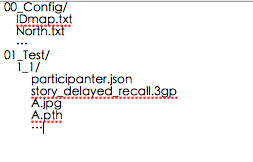
\includegraphics[clip]{OSS_format}
  \caption{阿里云OSS平台上数据存储格式}
\end{figure}

另外,患者的答案也用JSON格式化,也可以参加图3.8。

\subsection{大体框架设计}

系统主要由表达各题目的类和针对题目的界面Activity展示组成。这两个组成部分类似后台和前台,题目的类作为后台储存题目的逻辑部分,并完成一些判分的逻辑;界面Activity可以根据后台的逻辑展现题目,并完成一定的功能,传递数据给后台,让数据能存储到后台部分。这两部分相互独立,又相互依靠。

\subsubsection{题目的类}

\begin{figure}[h]
  \centering
  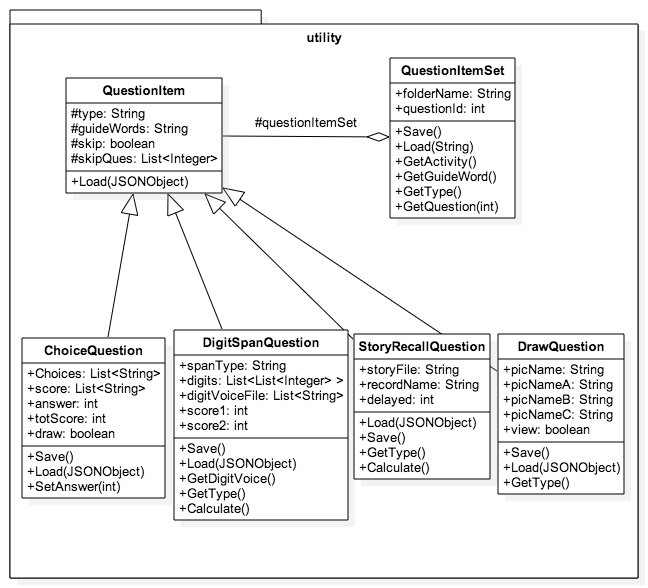
\includegraphics[width=13cm]{question-uml}
  \caption{题目类的UML图说明(部分)}
\end{figure}

所有的题目都基于一个叫做QuestionItem的基类(可见图3.10UML图),而继承的类可以根据其子成员type判断类型,这样即可以保证不同类型的题目可以按照自己的特征存储,保证了题目的完整性也保证了不会有信息冗余性;也可以保证前后台相互独立,可以分开开发。每个题目的类与对应题目格式化得到的JSON相对应,如ChoiceQuestion对应的选择题,成员变量Choices表示各选项的题目,成员变量score表示各选项的分数,成员变量answer表示患者选择的答案,成员变量totScore表示患者最终的得分,成员变量draw表示该选择题是否为图形选择题;而它的成员函数Save()为界面Activity提供了存储答案的接口,成员函数Load()可以从一个JSON中读入题目的各特征,成员函数SetAnswer()给界面Activity提供了传递患者答案的接口。

注:题目的类的集合QuestionItemSet作为整个APP的全局变量(Application)存在,方便整个APP运行过程中题目的读取和答案的保存。QuestionItemSet会在初始界面StartActivity里进行初始化。

\subsubsection{界面Activity}

\begin{figure}[h]
  \centering
  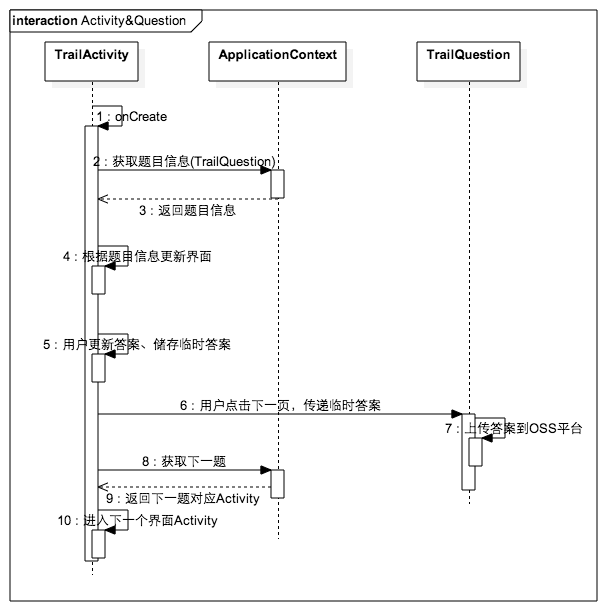
\includegraphics[width=13cm]{interaction}
  \caption{交互设计演示图(以单词配对题为例)}
\end{figure}

对应每个题目有一个对应的Activity来展现其题目,并实现收集数据、传递数据的功能。在初始化界面时,每个Activity从全局变量获取到需要展示的题目,根据其题目的类型和题目中的特征(如guideWords、选择题的选项)设置界面上的一些参数或一些需要播放的媒体文件(如录音题的一些音频)。然后根据用户对界面的操作(如对按钮的点击、修改文字等等)传递数据给后台,或是计算分数。当用户点击“下一页”时,根据后台给出的下一题类型,选出对应的Activity进行展示。

这样将题目的类、界面Activity分开,但相对应的设计,不仅使得开发过程中更为方便、不受干扰、便于调试,使得每种题目类型只需要实现一次,就可以“一劳永逸”;并且使得如果后续需要增加新的题目类型,也可以很方便的进行扩展性。


%%% Local Variables: 
%%% mode: latex
%%% TeX-master: t
%%% End: 

\newcommand{\tabincell}[2]{\begin{tabular}{@{}#1@{}}#2\end{tabular}}

\chapter{语音识别实验}

为了在目前市场中选择合适的语音识别接口作为支持本系统中语音识别的功能,以及了解目前开放的各个语音识别API的功能、性能、使用特性,设计了语音识别实验的内容。

\section{开放平台调查}

经过上网调查、查阅官方首先和说明文档,总结目前互联网市场上有如下开放的语音识别API:

\begin{table}[htbp]
\centering
\caption{开放语音识别API调查结果}
\label{tab:ParametersForPandR}
\begin{tabular}{ccccc}
\toprule[1.5pt]
{} & {\heiti 语音支持} & {\heiti 在线} & {\heiti 收费} & {\heiti 其他}\\\midrule[1pt]
百度云语音 & 中英 & \tabincell{c}{在线和离线\\都支持} & 免费 & \tabincell{c}{继承录音功能、语义理解\\上线后会有次数限制}\\
科大讯飞 & 中英 & 在线 & \tabincell{c}{含免费\\部分} & \tabincell{c}{有语义解析功能、降噪\\大量使用后会有次数限制}\\
\tabincell{c}{Google\\语音识别} & 中英 & 在线 & 免费 & \tabincell{c}{非针对移动应用\\必须FLAC格式文件}\\
搜狗语音云 & 中文 & 在线 & 免费 & \tabincell{c}{服务次数上限:1000/一天\\集成录音\\降噪网络通讯和状态通知}\\
微信语音平台 & 中英 & 在线 & 收费 & -\\
云知声语音云 & 中文 & 在线 & 收费 & -\\
语意果 & 中文 & 在线 & 收费 & -\\
\bottomrule[1.5pt]
\end{tabular}
\end{table}

\section{实验设计和说明}

考虑到设计系统需要英文语音识别、但也需要在未来开发中文系统,根据该需求和上一小节的调研结果,一共选择了三个备选公共平台API做测试(百度云、科大讯飞、Google语音识别)。由于提供的接口不同,Google语音识别API测试的方法为合成录音文件为FLAC格式后传输后得到结果,其余API(百度云和科大讯飞)测试为电脑播放录音,手机端得到测试结果。

针对《脑健康系统研究》中的语音题,设计测试录音如下:

\begin{itemize}
\item 录音A:中文单词测试:金属,哭泣,黑暗,北方,学校,玫瑰,向上,英尺,苹果,钢笔;
\item	录音B:中文连续测试:草原上有对狮子母子,小狮子问母狮子:“妈妈,幸福在哪里?”母狮子说:“幸福就在你的尾巴上呀”于是小狮子不断追着尾巴跑,但始终咬不到。母狮子笑道:“傻瓜!幸福不是这样得到的。只要你昂首向前走,幸福就会一直跟着你。”\footnote{该小故事转自百度};
\item 录音C:英文单词测试,metal,cry,dark,south,school,rose,up,inch,apple,pen(原问卷中原题);
\item 录音D:英文连续测试:Anna, of South Boston, employed as a scrub woman in an office building, reported at the City Hall Station that she had been held up, on State Street, the night before, and robbed of fifteen dollars. She had four little children, the rent was due, and they had not eaten for two days. The officers, touched by the woman’s story, made up a purse for her.(原问卷中原题);
\item 每个录音会播放三遍:第一遍为遍正常音量、第二遍为遍音量较小、第三遍为人工增加噪声的正常音量;
\item 录音由本人录制,在英语上可能有一些词语发音不标准导致结果有偏差。
\end{itemize}

\section{实验结果}

\begin{table}[htbp]
\centering
\caption{开放语音识别API调查结果}
\label{tab:ParametersForPandR}
\begin{tabular}{ccccc}
\toprule[1.5pt]
{} & {\heiti 中文单词} & {\heiti 中文连续} & {\heiti 英文单词} & {\heiti 英文连续}\\\midrule[1pt]
百度云语音 & \tabincell{c}{正常音量和加噪\\下非常顺利通过\\测试\\小音量下错误率\\比较高 5/10} & \tabincell{c}{正常音量加噪下\\错了一句话\\大体识别正确\\小音量下几乎不\\能用} & \tabincell{c}{正常音量:识别\\对了7/10\\噪音:5/10\\小音量:3/10} &  \tabincell{c}{正常音量情况下\\文字大体长得差\\不多(语法基本\\能识别正确),关\\键词有错误情况\\噪声情况下略差\\小音量几乎不能用}\\
科大讯飞 & \tabincell{c}{正常音量下顺利\\通过测试\\噪声环境下有一\\个词语错误\\小音量下错误率\\较高 5/10} & \tabincell{c}{正常音量和加噪\\情况下顺利通过\\测试小音量下错误率\\很高} & \tabincell{c}{正常音量:8/10\\噪音:7/10\\小音量:3/10\\} &  \tabincell{c}{和百度云的情况\\相近}\\
Google语音识别 & \tabincell{c}{正常10/10\\噪声9/10\\因为是文件传\\输,小音量没有\\很大影响8/10} & \tabincell{c}{加噪情况下错了\\2句话\\小音量下错了1句}  & \tabincell{c}{10/10\\小音量:8/10}  & \tabincell{c}{语法基本正确\\关键词基本上都\\差不多}\\
\bottomrule[1.5pt]
\end{tabular}
\end{table}

实验结果可见表4.2。通过对实验结果的分析,可以得出一下这些结论:

\begin{itemize}
\item 百度的sdk中有一些模版的接口,比较适用于android开发;
\item	在中文处理上,百度和讯飞做得还算不错,正确率能达到90%以上。Google的稍逊;
\item 但是在英语处理上,百度和讯飞在语法的识别上还是可以,但是在关键词的识别上稍微差一些;
\item 小音量的情况下,百度和讯飞处理都非常不好;
\item 总体来说,百度和讯飞在测试结果上没有明显的差异。
\end{itemize}

\section{实验结论}

\begin{itemize}
\item 有三个比较合适(免费、支持中英文)备选API:百度、讯飞、google语音识别;
\item	中文处理上百度云和科大讯飞功能强于google语音识别,加噪的条件下准确率90%以上;
\item 英文处理上,百度云和科大讯飞对语法的识别还算可用,但有关键词识别错误(可能测试的发音有问题);
\item 小音量下API的性能很差完全不能使用;
\item Google语音的API非针对移动端,考虑到接到Android开发上可能会非常不方便,百度云和科大讯飞的总体上来说性能接近。由于百度云的应用接口更容易使用,选择使用百度云的语音识别SDK
\end{itemize}


%%% Local Variables: 
%%% mode: latex
%%% TeX-master: t
%%% End: 

\chapter{模块实现}

每个模块对应了一类题型,即一个Activity和其对应的Question。在这次设计中,充分运用了Android的界面设计(即每个Activity可以对应一个XML文件),这样可以加速程序加载,也可以通过界面中组件的ID进行个性化设置。

\section{登陆模块}

\begin{figure}[h]
\centering%
\begin{subfigure}{6cm}
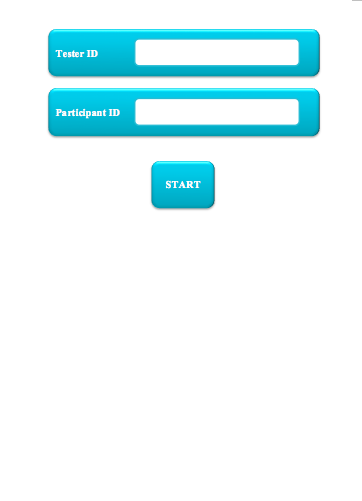
\includegraphics[width=6cm]{loginD}
\caption{登陆模块-设计}
\end{subfigure}
\hspace{4em}%
\begin{subfigure}{6cm}
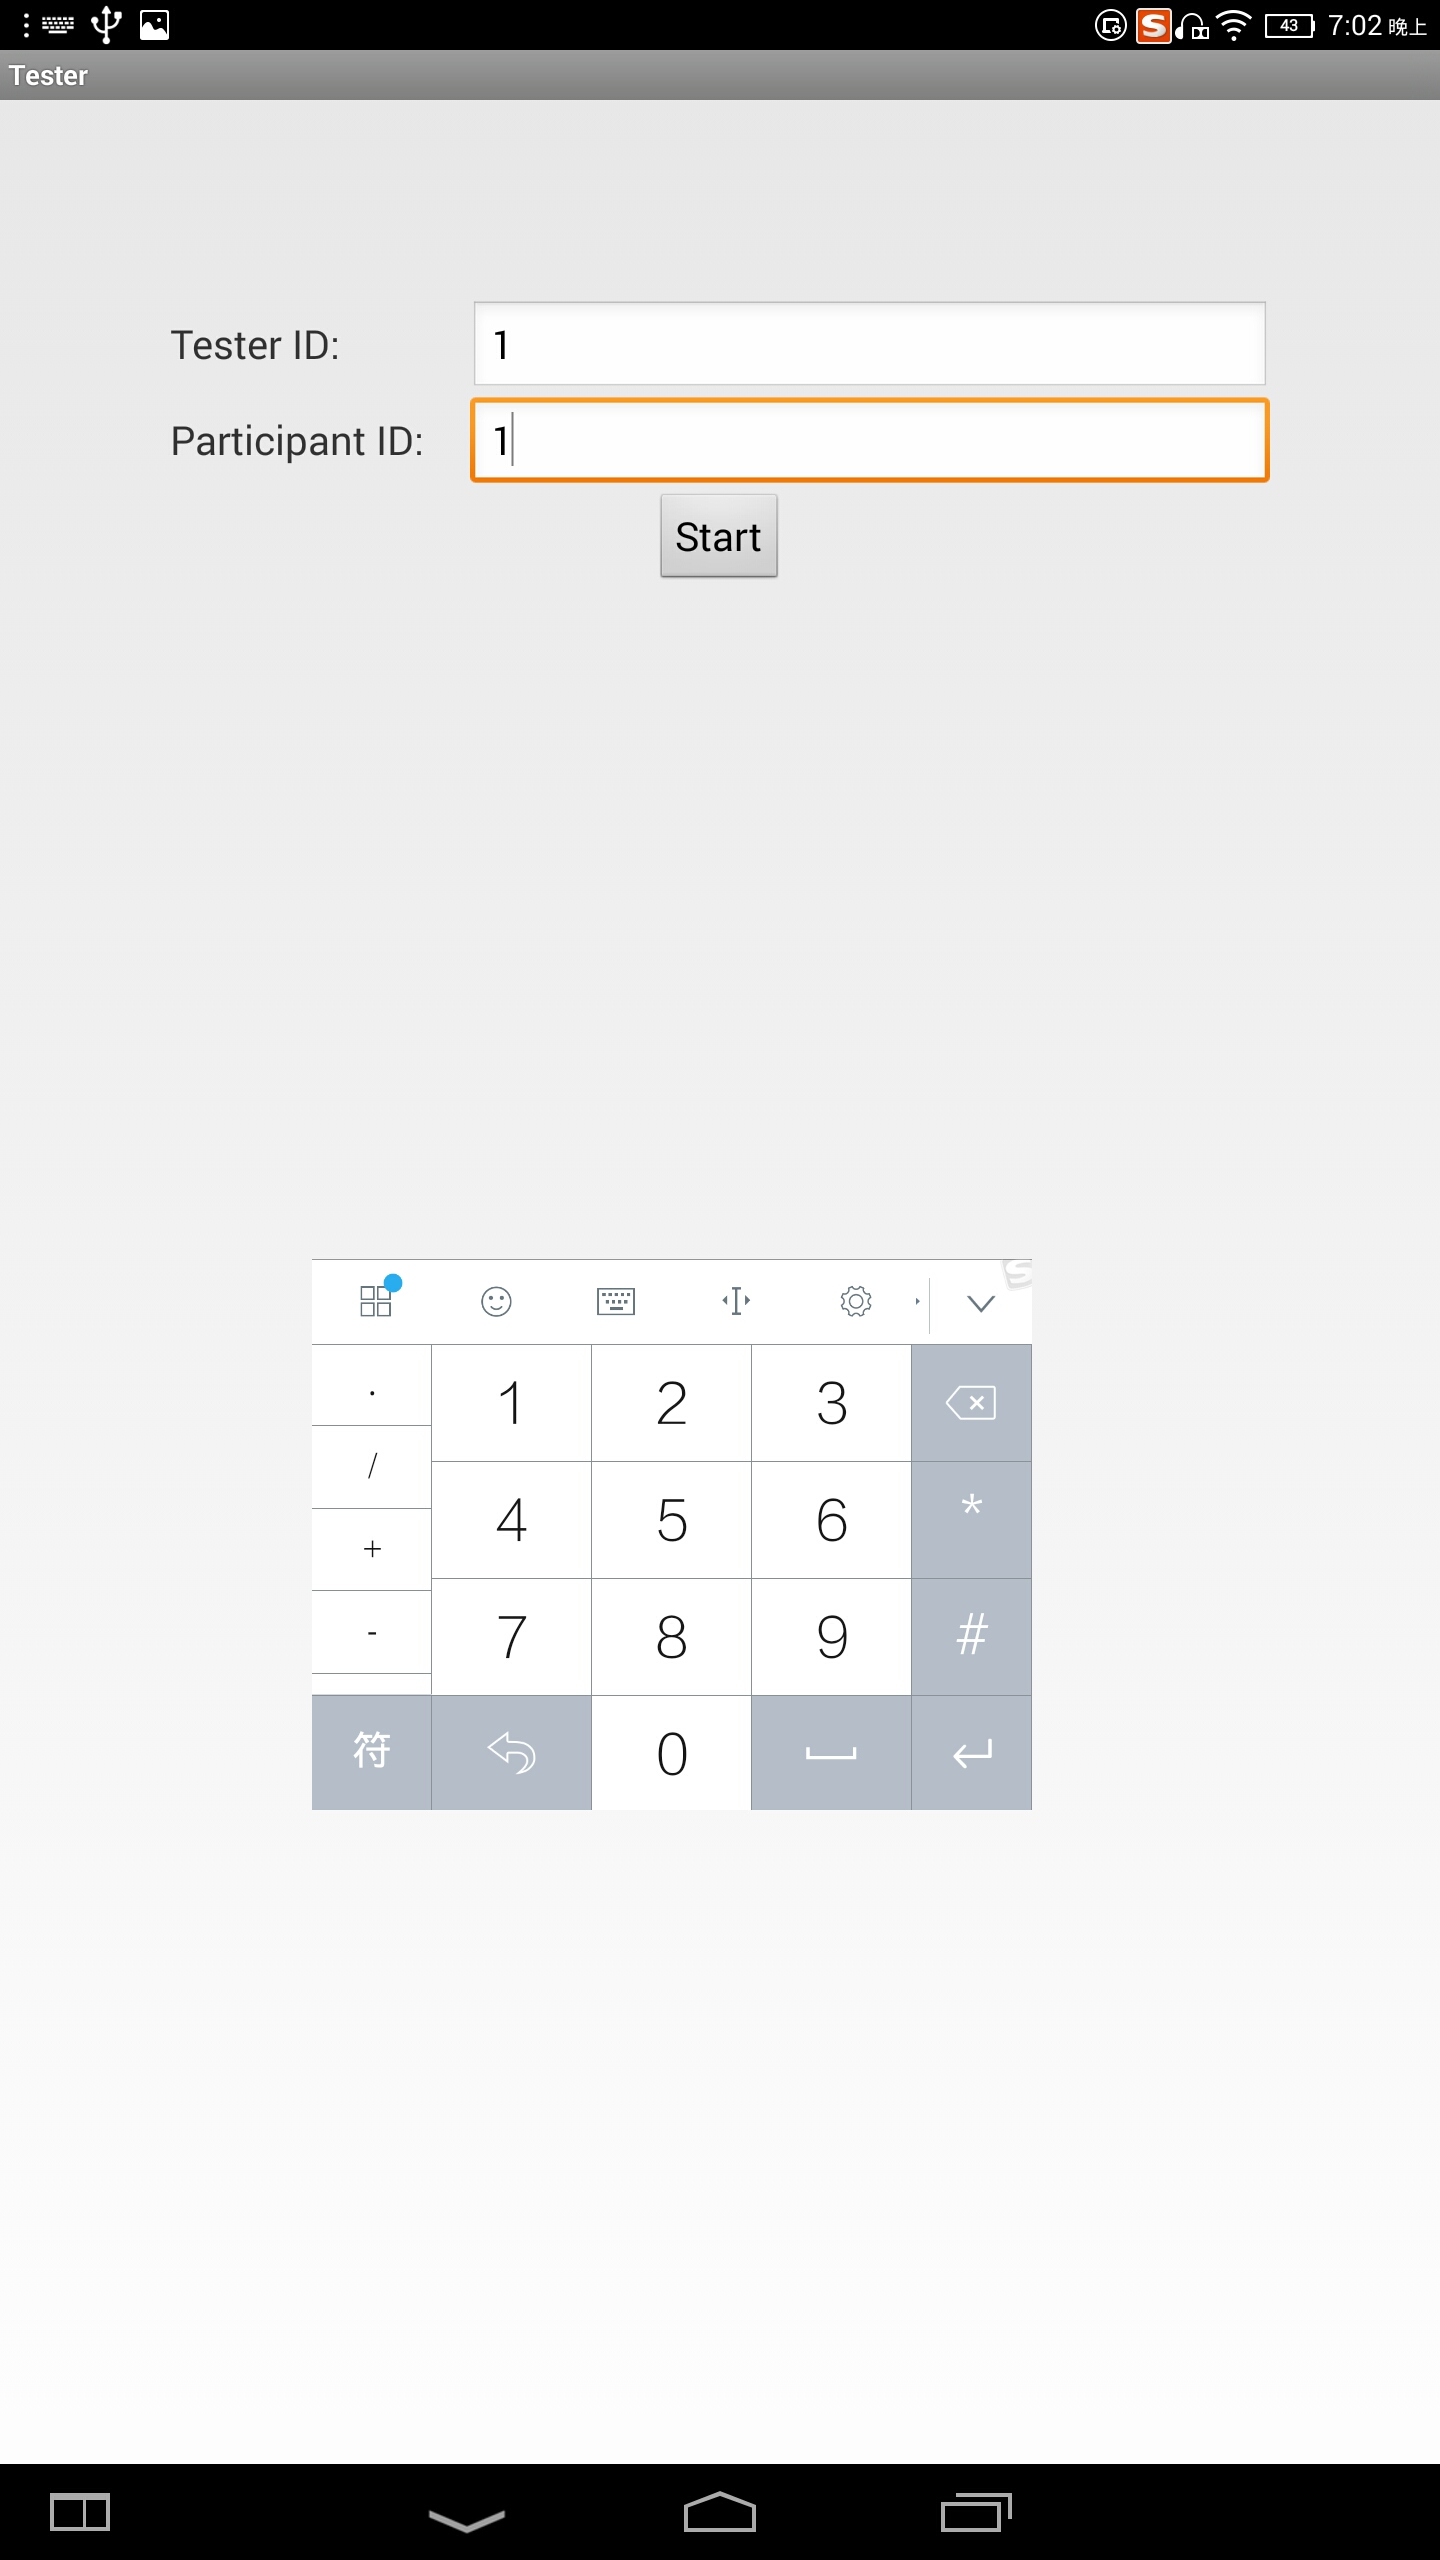
\includegraphics[width=6cm]{login}
\caption{登陆模块-最终实现}
\end{subfigure}
\caption{登陆模块设计和最终实现图}
\label{fig:big1-subfigure}
\end{figure}

登陆模块是整个APP的开始,三个版本的APP中都会包括这个模块,在这个模块中会对程序所有需要的配置和变量进行初始化(所有的题目以及需要评分的答案)。而这个模块的主要功能为确定医生ID和病人ID设计,这样可以使测试得到的数据与日期、病人一一对应,其中在数据库中已经建立了匹配的字符串对(储存在OSS平台上的配置文件目录下的IDmap.txt里),生成规则由波士顿大学给出。该模块的逻辑比较简单,即获取界面上用户输入的TesterID和ParticipanterID后连接数据库,与数据库中的配对进行匹配即可,若成功,则进入第一题,否则弹出一个错误提示对话框,说明数据库中没有对应匹配,要求用户重新输入再次尝试。

\section{故事复述题模块}

\begin{figure}[h]
\centering%
\begin{subfigure}{6cm}
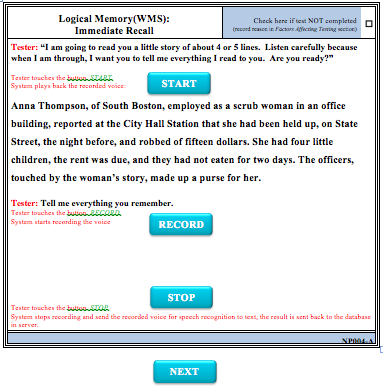
\includegraphics[width=6cm]{storyD}
\caption{数字串复述题-设计}
\end{subfigure}
\hspace{4em}%
\begin{subfigure}{6cm}
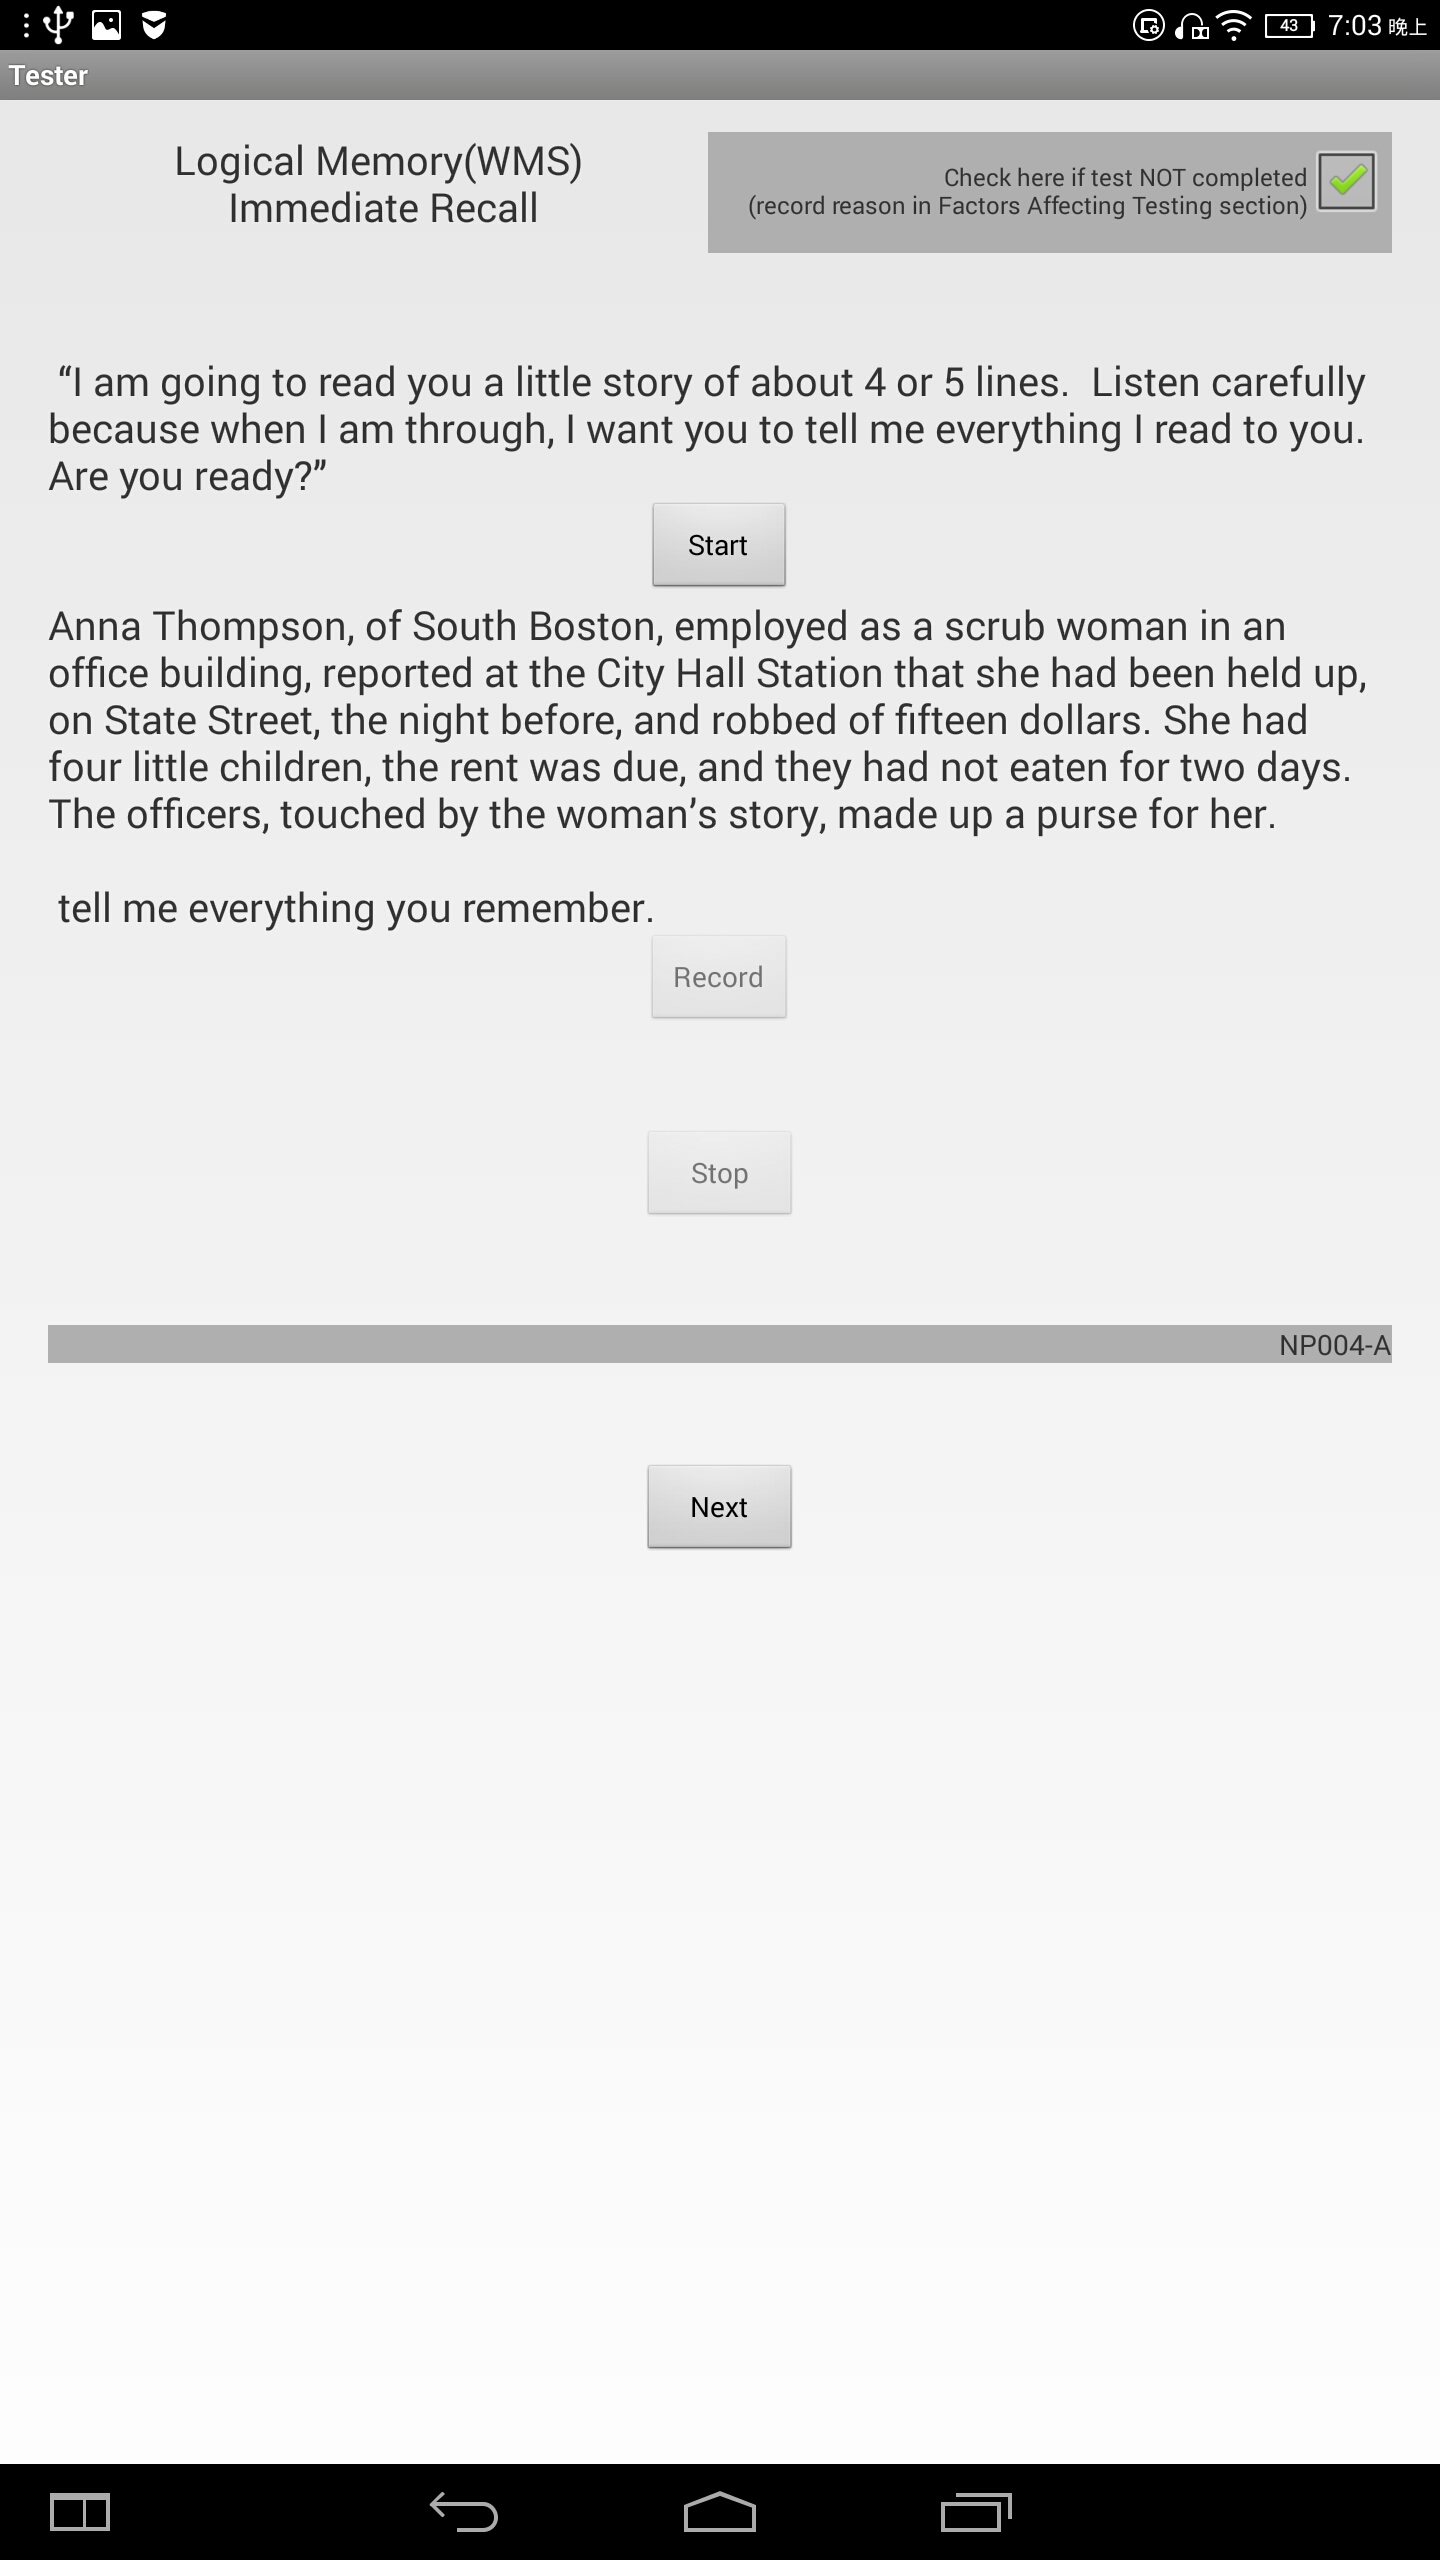
\includegraphics[width=6cm]{story}
\caption{故事复述题-最终实现}
\end{subfigure}
\caption{故事复述题设计和最终实现图}
\label{fig:big1-subfigure}
\end{figure}

故事复述题包括在线测试版和离线打分版两部分。对于在线测试版,除了界面上需要有提示词之外,需要有播放录音、以及音频录制的功能。这里直接使用了Android自带的MediaPlayer和MediaRecorder,根据题目JSON中的信息,查找已经放在工程中对应的音频文件,点击Start按钮后进行播放;同样也根据JSON中录音名的信息,在平板电脑的根目录下创建对应的临时文件,并在用户点击下一题时上传该文件,然后删除这个临时文件。这里为了引导用户按照顺序(播放录音、录制、停止录制),为按钮设置了可按的顺序(即开始只能播放录音、在播放完录音后才能开始录制音频,在开始录音后才能选择停止录制)。

\begin{figure}[h]
\centering%
\begin{subfigure}{6cm}
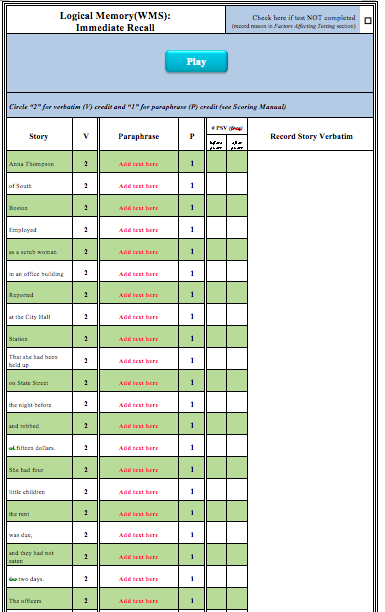
\includegraphics[width=6cm]{storyscoreD}
\caption{数字串复述题离线打分版-设计}
\end{subfigure}
\hspace{4em}%
\begin{subfigure}{6cm}
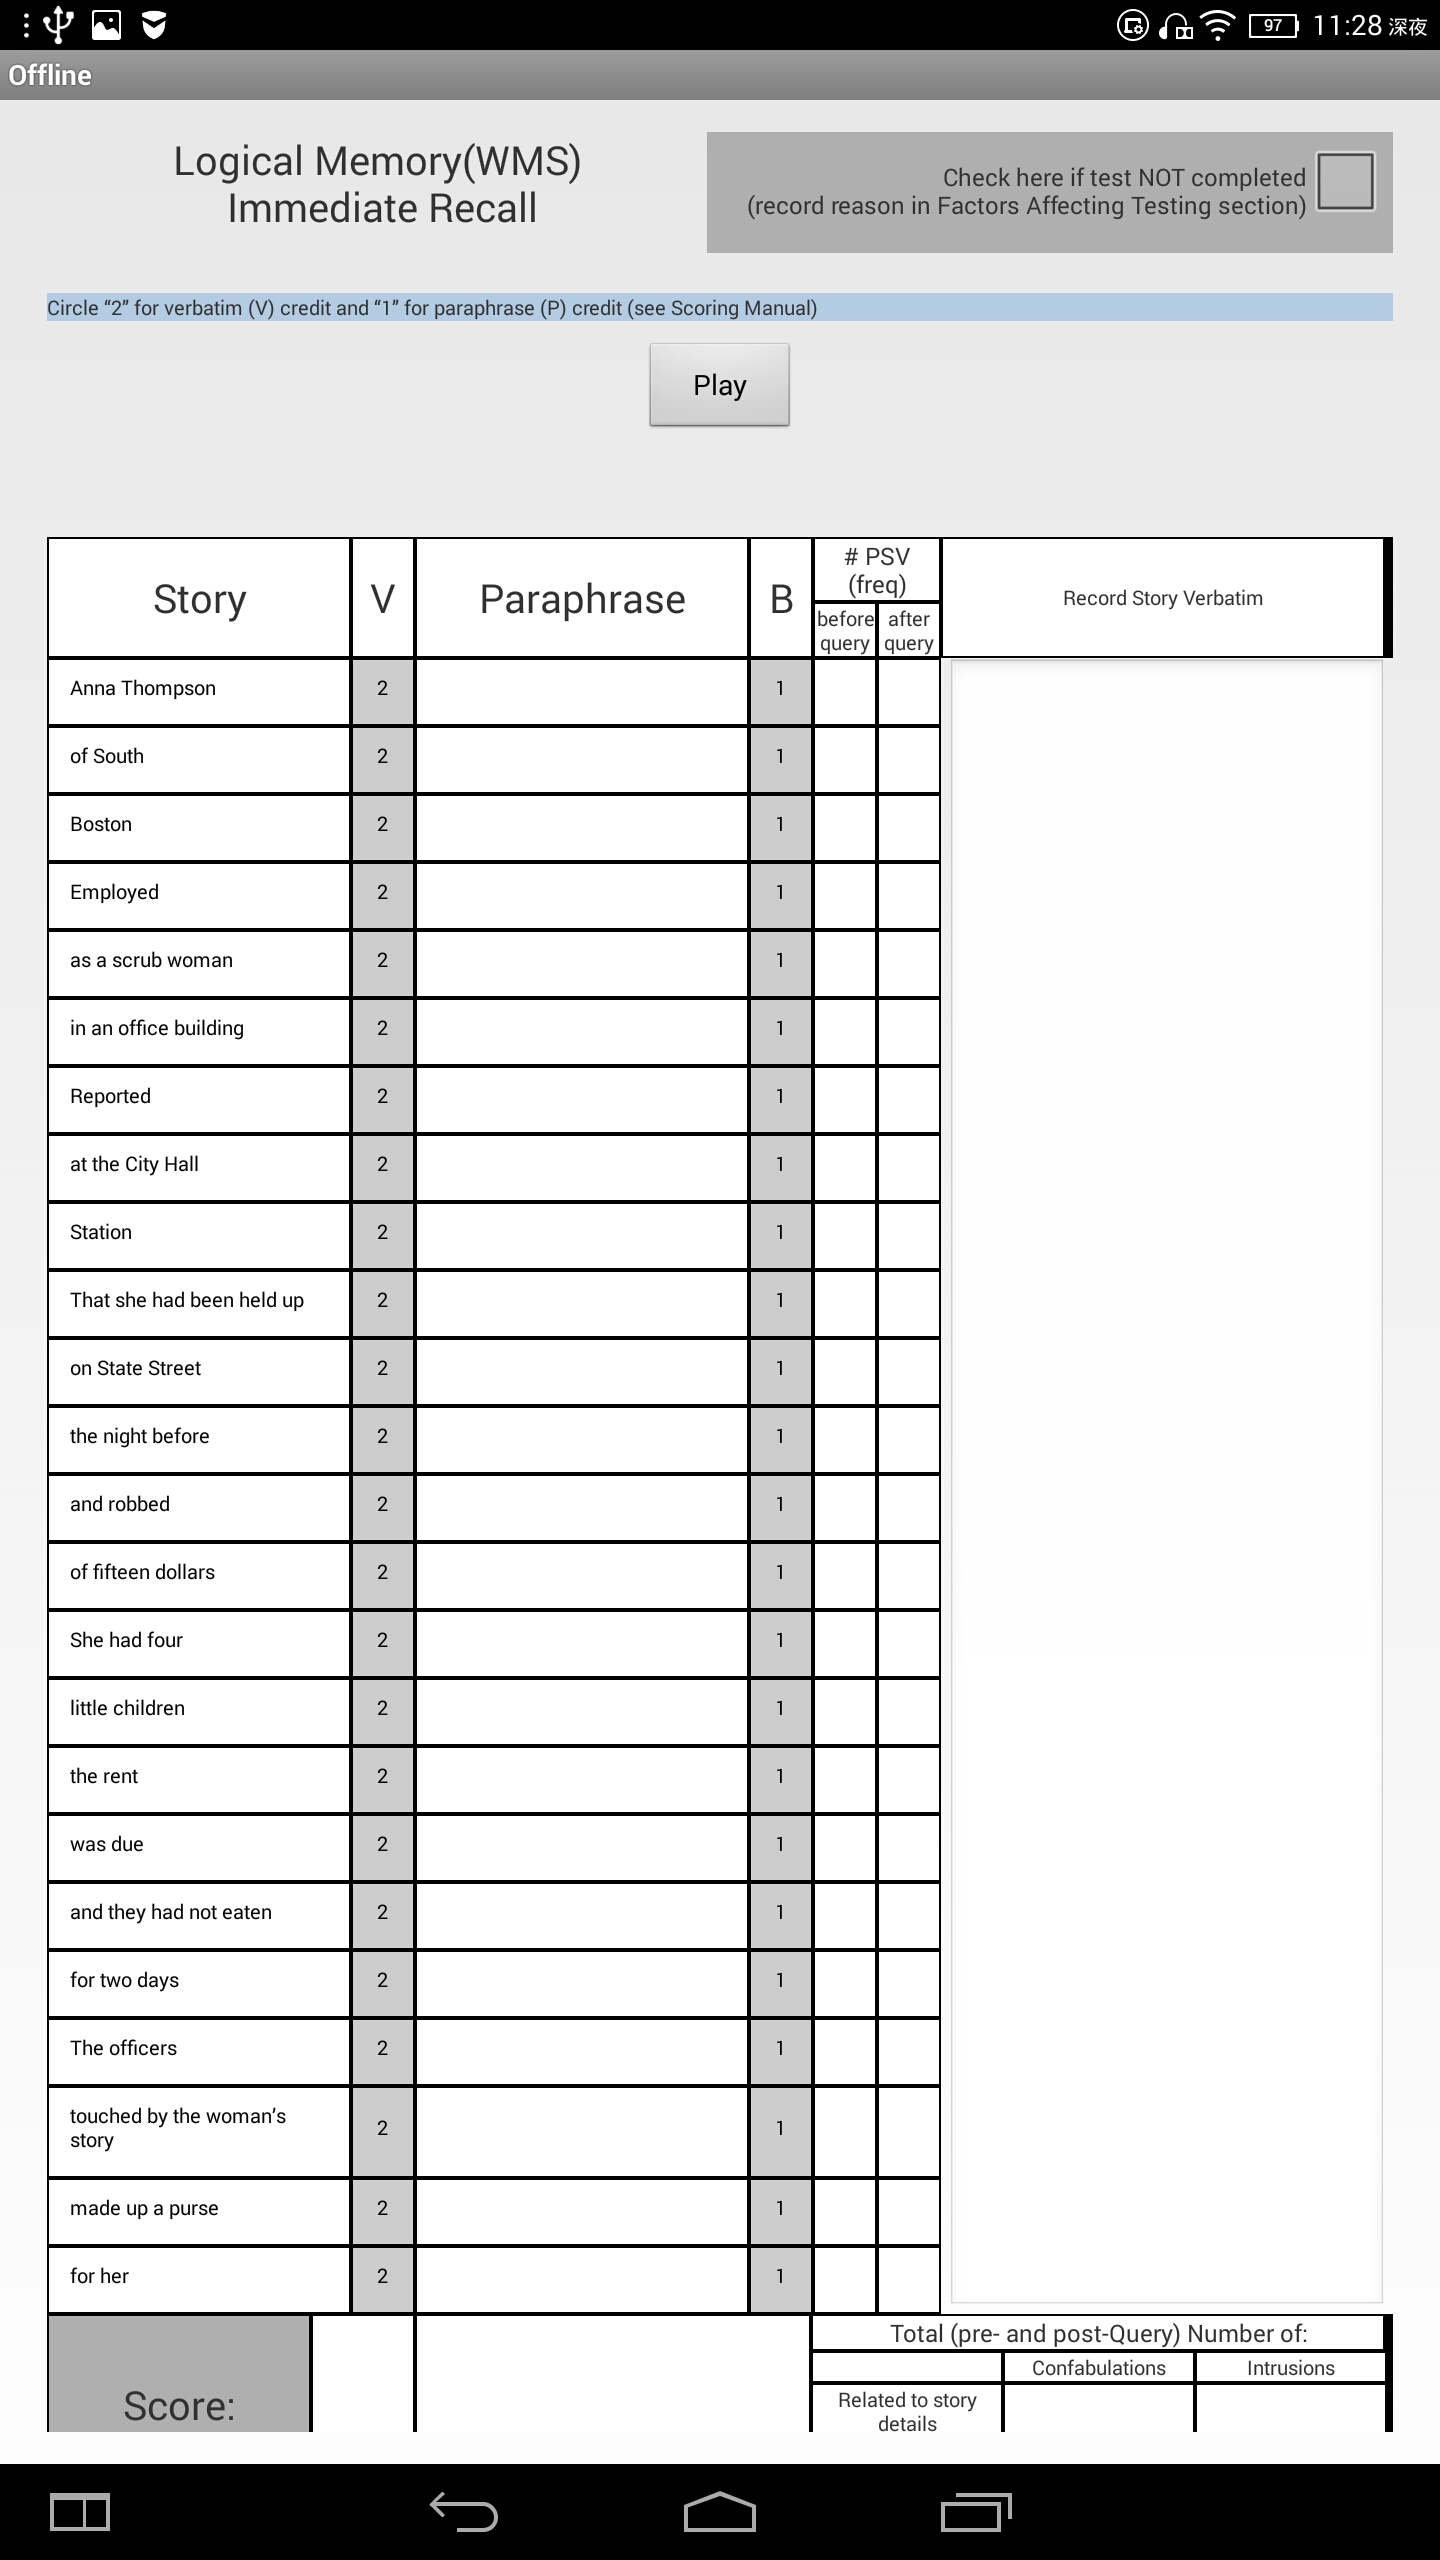
\includegraphics[width=6cm]{storyscore}
\caption{故事复述题离线打分版-最终实现}
\end{subfigure}
\caption{故事复述题离线打分版设计和最终实现图}
\label{fig:big1-subfigure}
\end{figure}

离线打分版需要展示所有打分项,以及播放录音、识别录音信息等功能。在界面加载时,会根据题目JSON文件从OSS将需要的媒体文件下载(播放的录音),而题目的答案在初始APP已经更新。打分项的每一行都用自定义的SingleStoryScoreView作为界面组件,这个组件包括了故事、打分按钮和打分方框,独立定义组件是为了避免过多重复代码的写入。在计算分数时,会统计每个SingleStoryScoreView的得分再总和。播放录音同样使用Android自带的MediaPlayer。录音识别使用了百度语音识别的接口(在上一章的内容中已经介绍),通过监听回调结果并显示在界面,辅助用户快速做评分。

\section{画图题模块}

\begin{figure}[h]
\centering%
\begin{subfigure}{6cm}
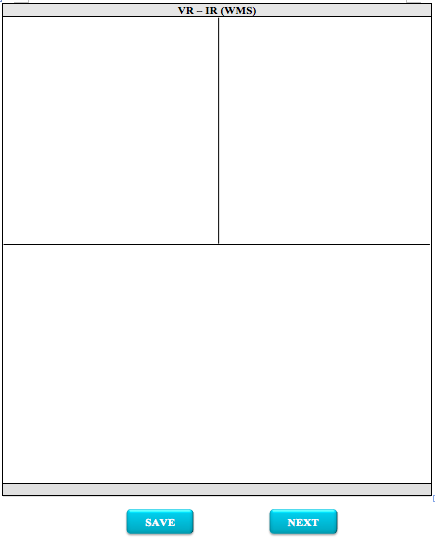
\includegraphics[width=6cm]{drawD}
\caption{画图题病人版-设计}
\end{subfigure}
\hspace{4em}%
\begin{subfigure}{6cm}
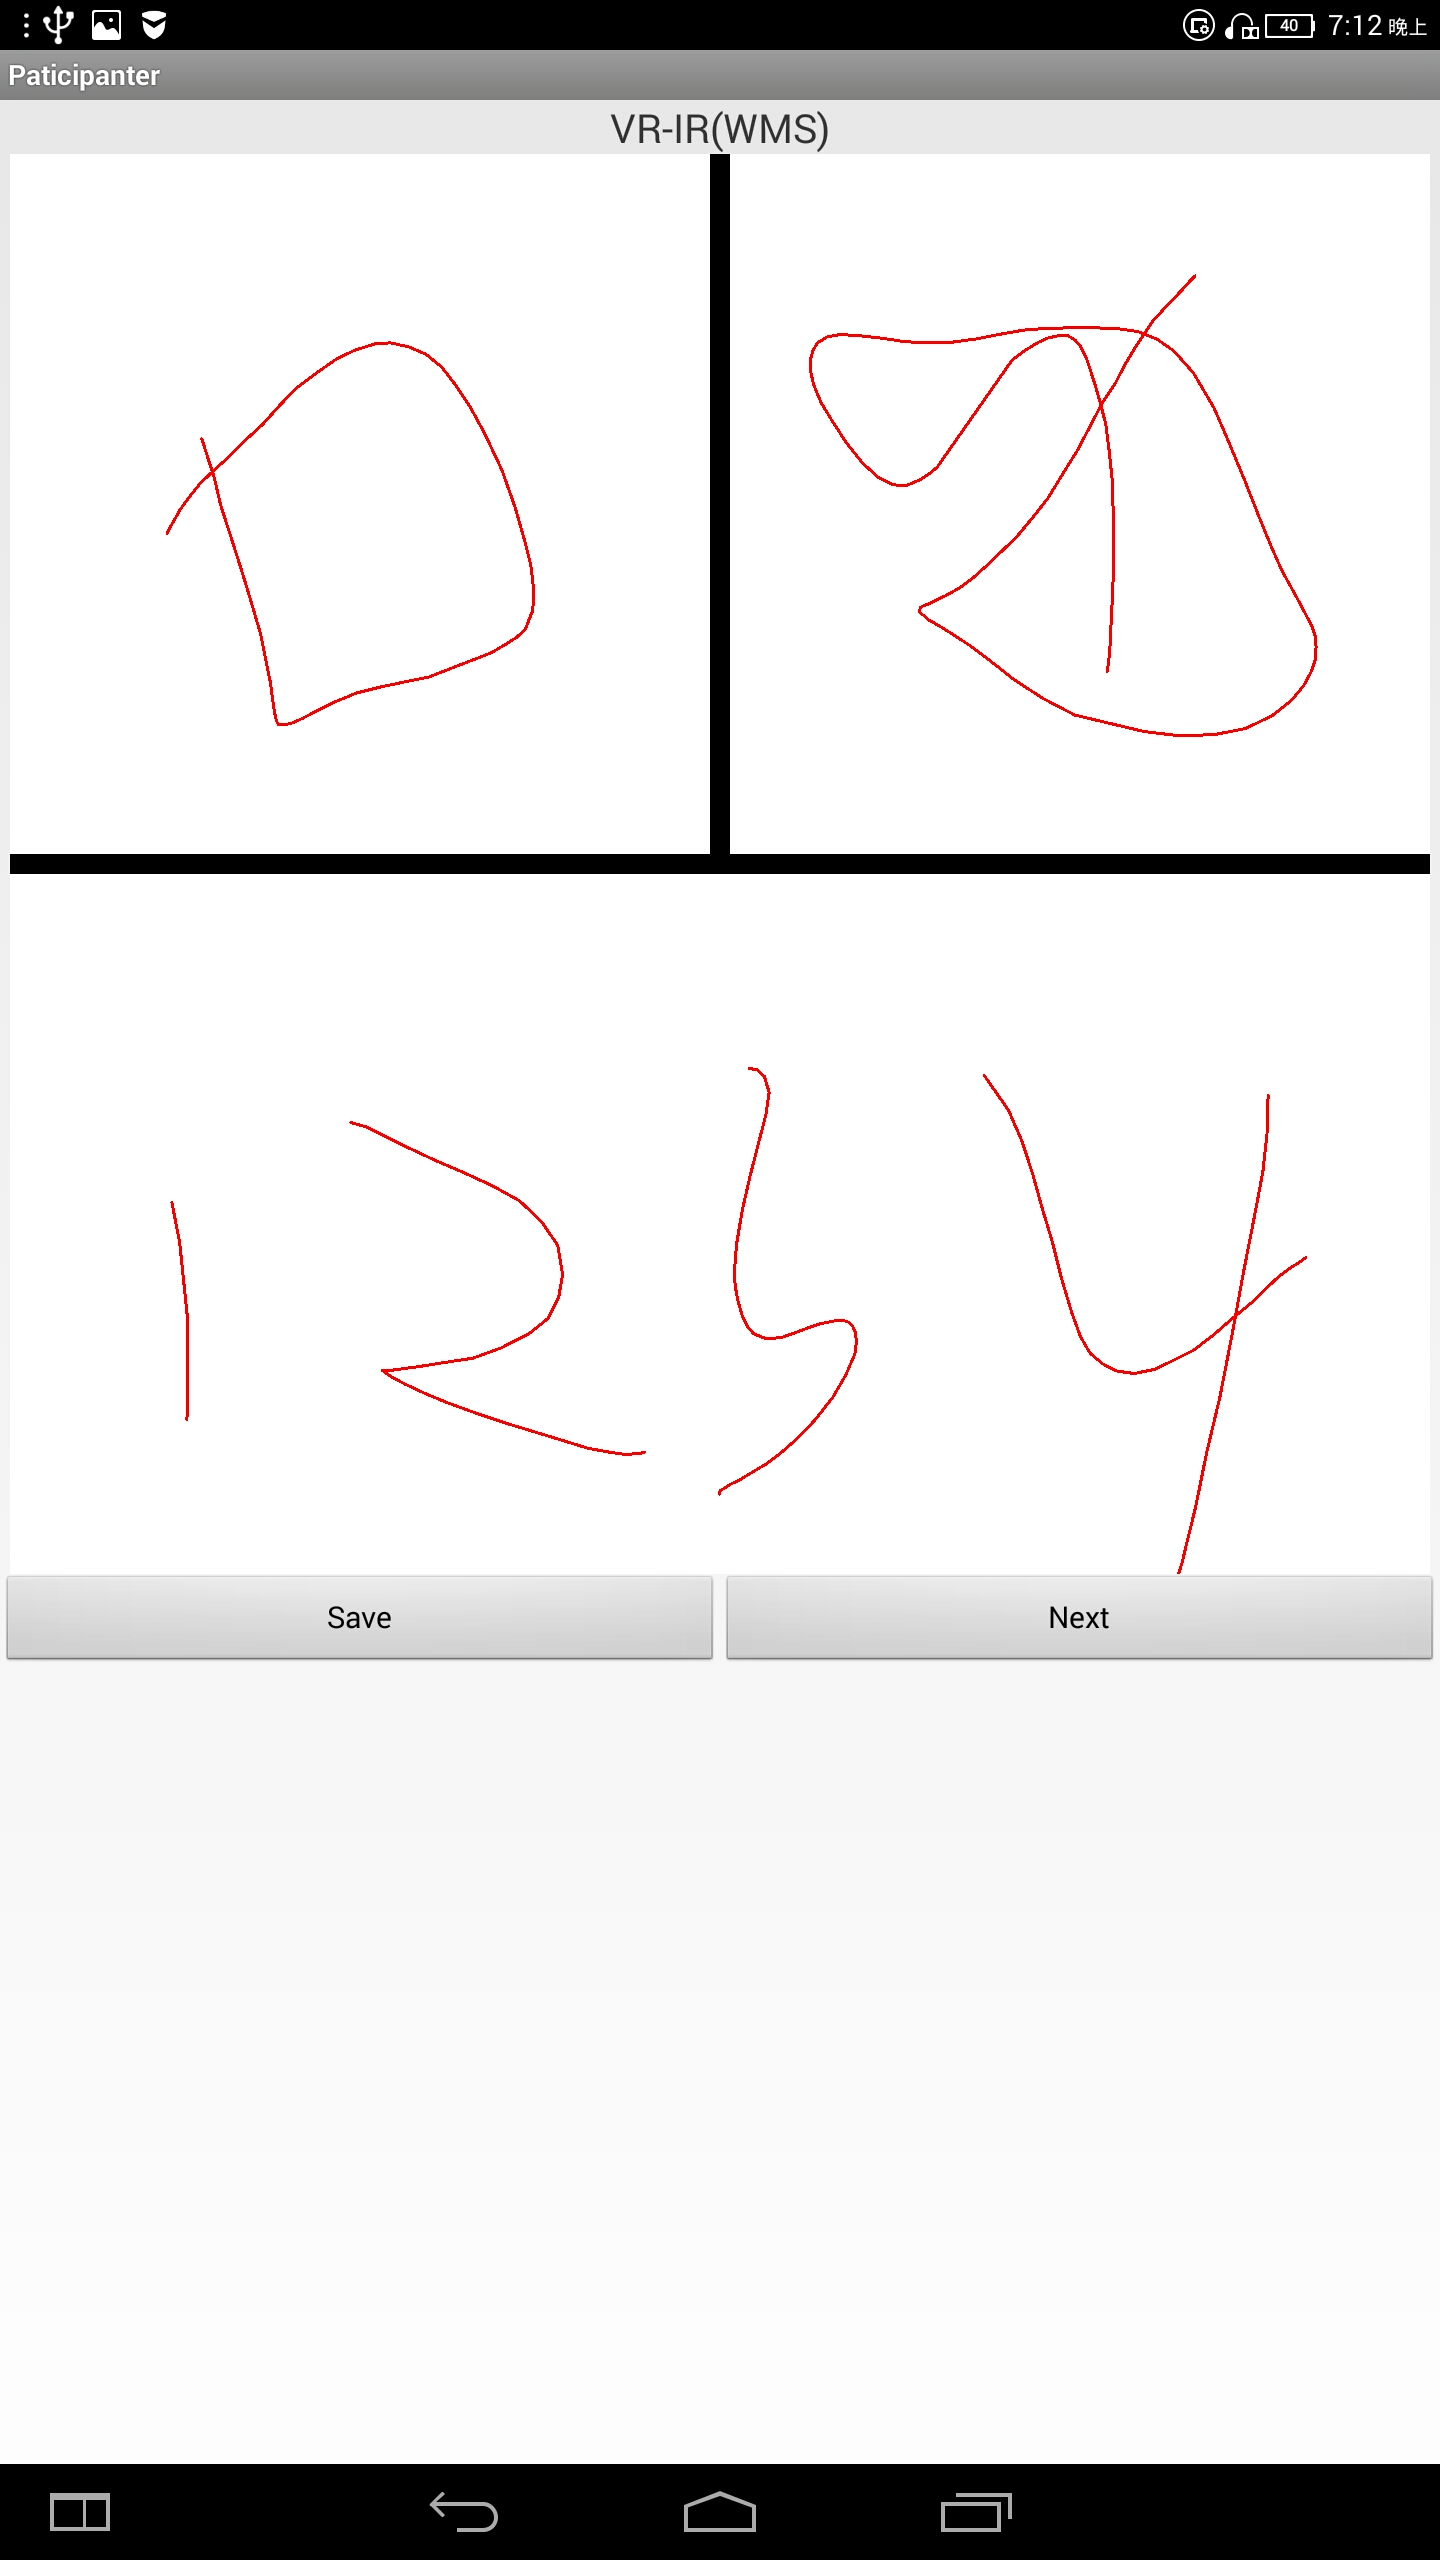
\includegraphics[width=6cm]{draw}
\caption{画图题病人版-最终实现}
\end{subfigure}
\caption{画图题设计和最终实现图}
\label{fig:big1-subfigure}
\end{figure}

画图题包括了在线病人版、在线医生版和离线打分版三个部分。为了还原和纸板一样的用户体验(即医生和用户都需要有“平板”在面前),在在线病人版和在线医生版中都存在。病人版主要是为了让病人能够画图,并能够记录下病人画图的轨迹。由于有些题目是有顺序的,这里也加入了顺序的概念,即界面上只有一处是可以画的,只有当病人点击“下一个”时,接下来需要画的部分才会打开。绘画过程主要用了Android自带的Paint工具,开启绘画的线程接收用户的点击并描绘和记录轨迹,在平板电脑的根目录下创建与题目JSON对应的临时文件,然后根据用户的选择进行上传。

在线医生版主要的功能是能够展示题目提示和限时展示图片,在展示图片时需要做到屏幕上只有图片而没有其他东西。这里的模块设计也完全按照顺序,根据用户的点击开启Handler计时、显示图片并隐藏其他内容,当Handler显示时间已经到时再恢复显示其他内容。

\begin{figure}[h]
\centering%
\begin{subfigure}{6cm}
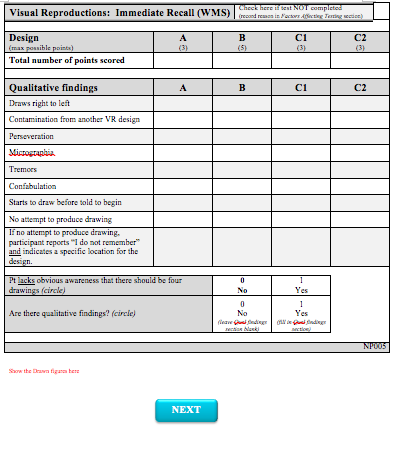
\includegraphics[width=6cm]{drawscoreD}
\caption{画图题离线打分版-设计}
\end{subfigure}
\hspace{4em}%
\begin{subfigure}{6cm}
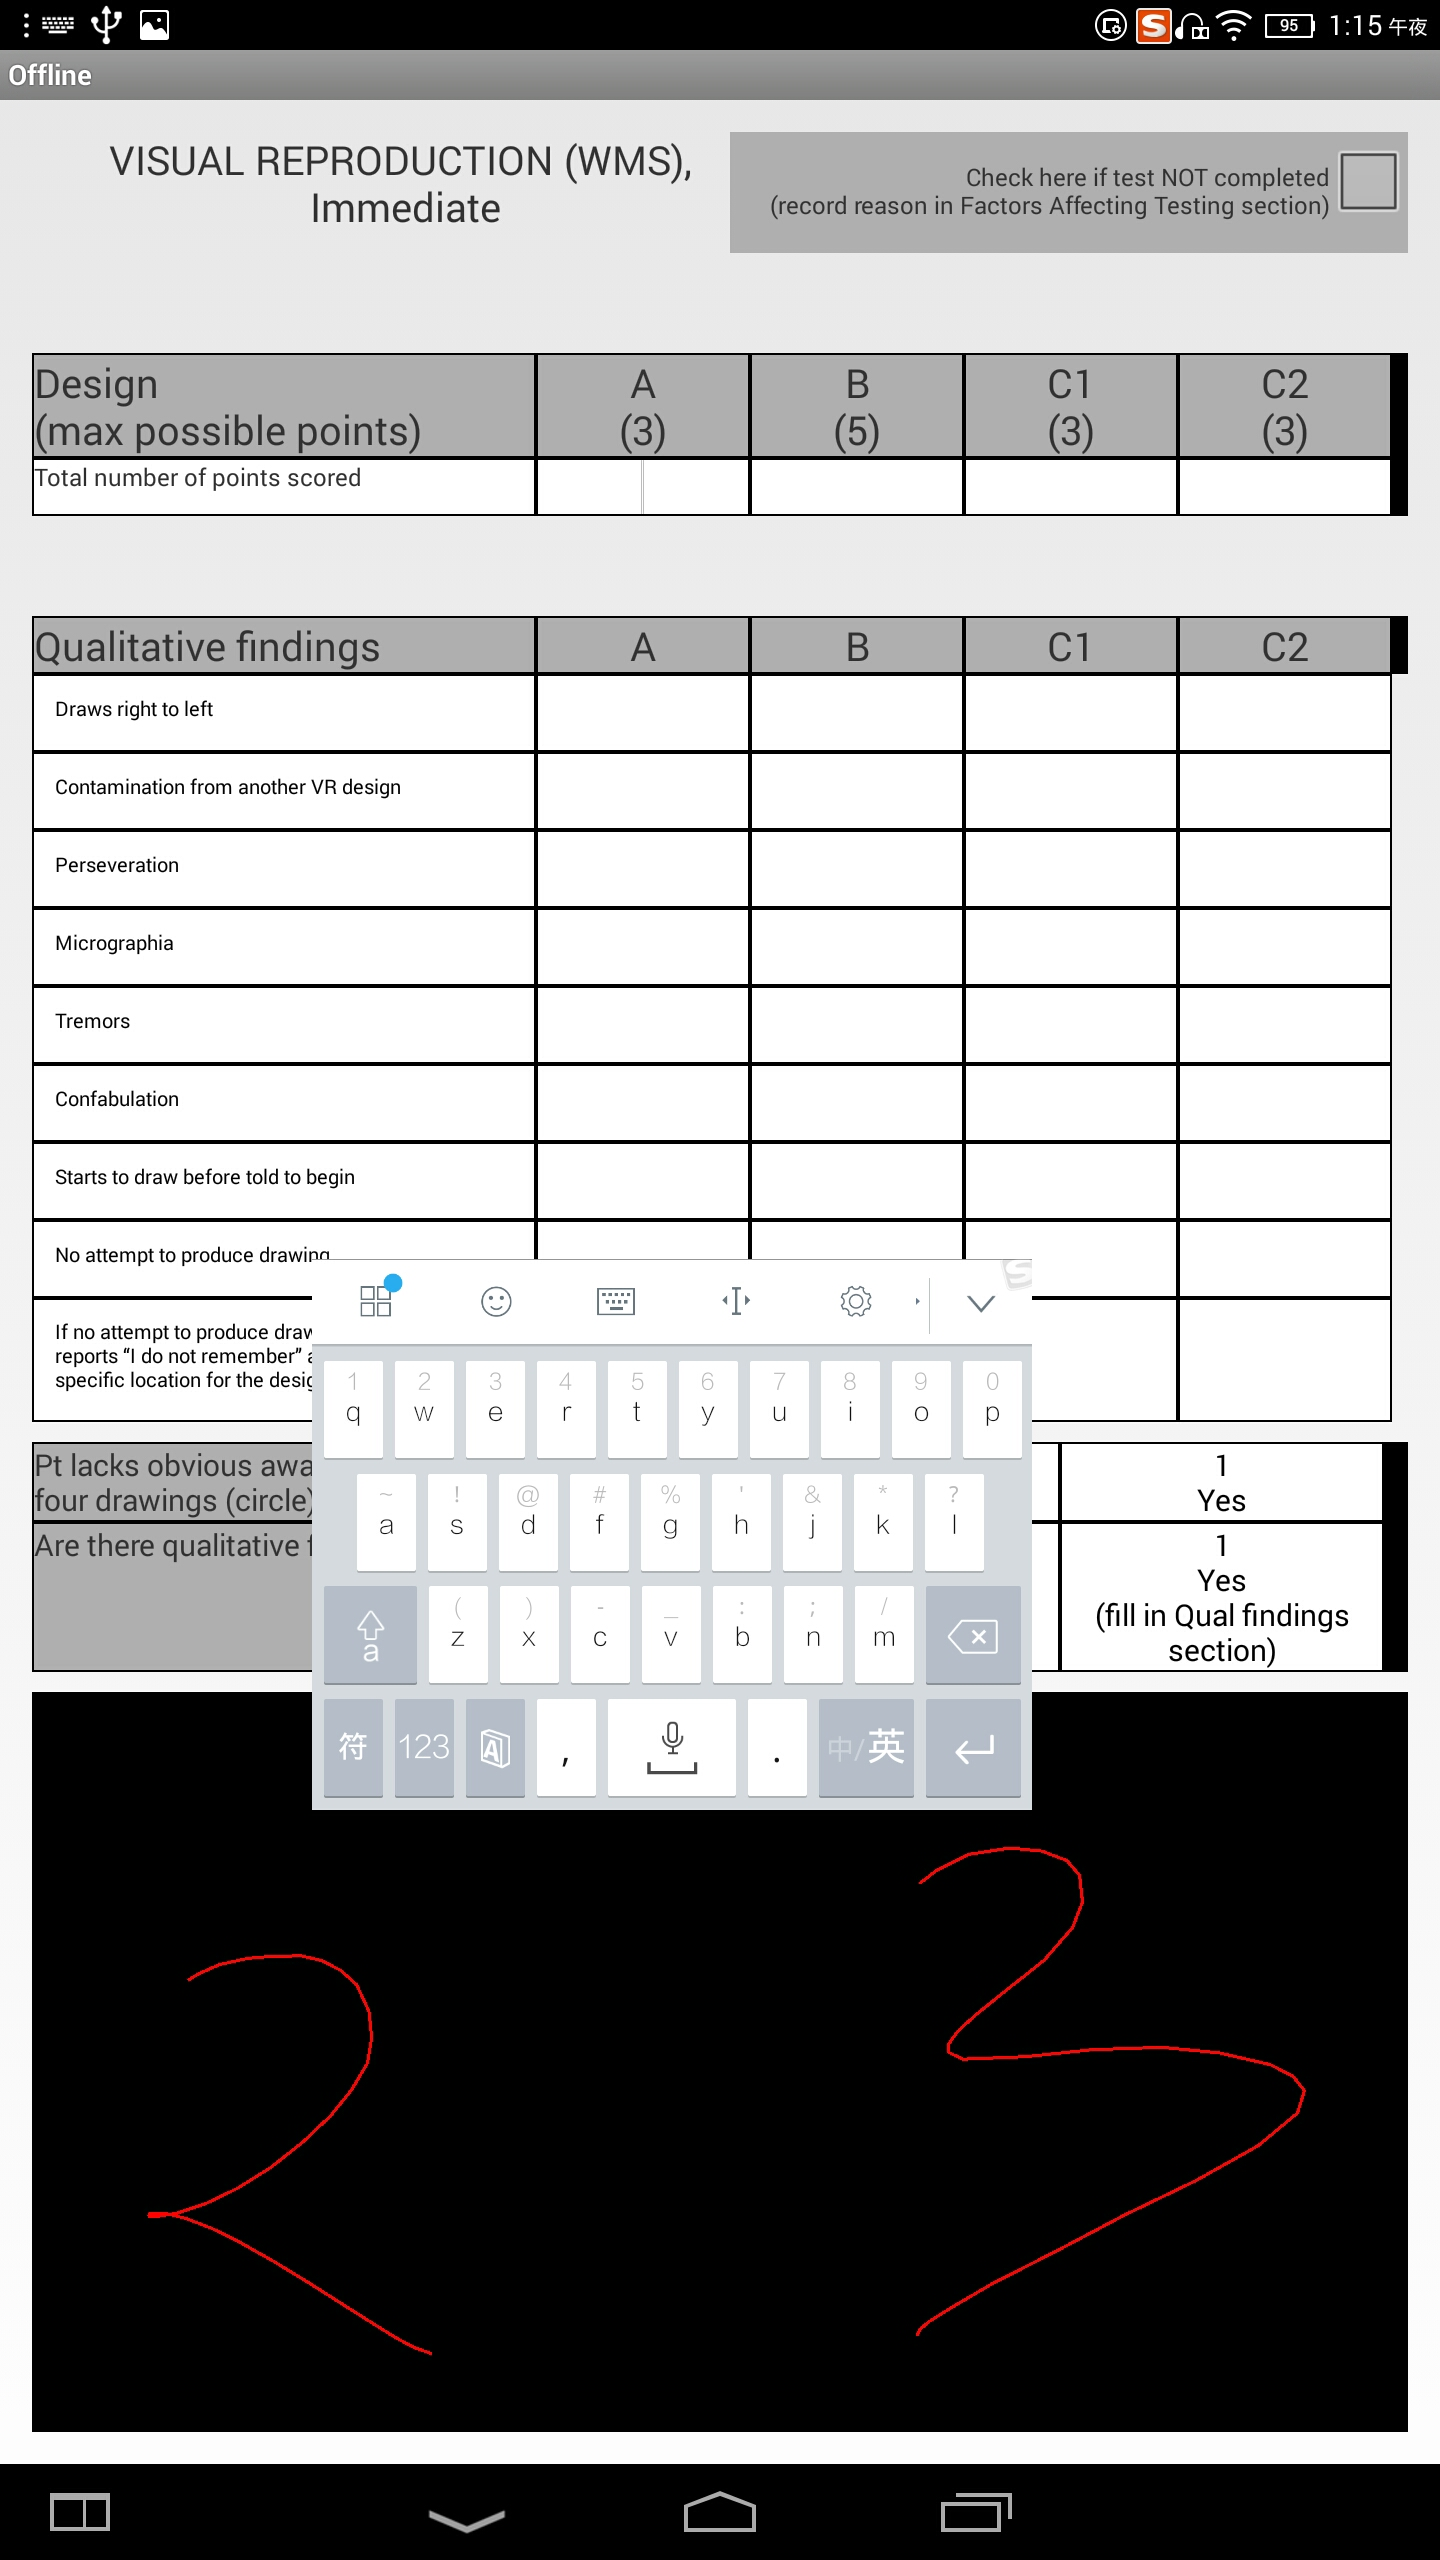
\includegraphics[width=6cm]{drawscore}
\caption{画图题离线打分版-最终实现}
\end{subfigure}
\caption{画图题离线打分版设计和最终实现图}
\label{fig:big1-subfigure}
\end{figure}

离线打分版只需展示各打分选项和图片即可。界面加载时会从OSS平台下载所需资源(用户所画的图)。打分选项的实现与故事复述题离线打分版的打分选项的实现类似,每一个打分选项用自定义的界面组件SingleDrawScoreView表现,统计分数时统计每一个组件的分数并取和。图片的显示运用了ImageView来展示。

\section{单词对复述题模块}

\begin{figure}[h]
\centering%
\includegraphics[width=13cm]{trailA}
\caption{单词对复述题逻辑流程图}
\label{fig:big1-subfigure}
\end{figure}

\begin{figure}[h]
\centering%
\begin{subfigure}{6cm}
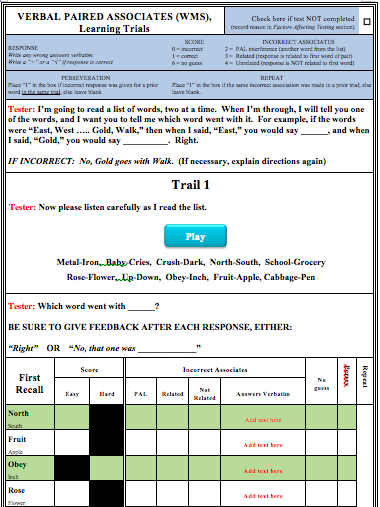
\includegraphics[width=6cm]{trailerD}
\caption{单词对复述复述题-设计}
\end{subfigure}
\hspace{4em}%
\begin{subfigure}{6cm}
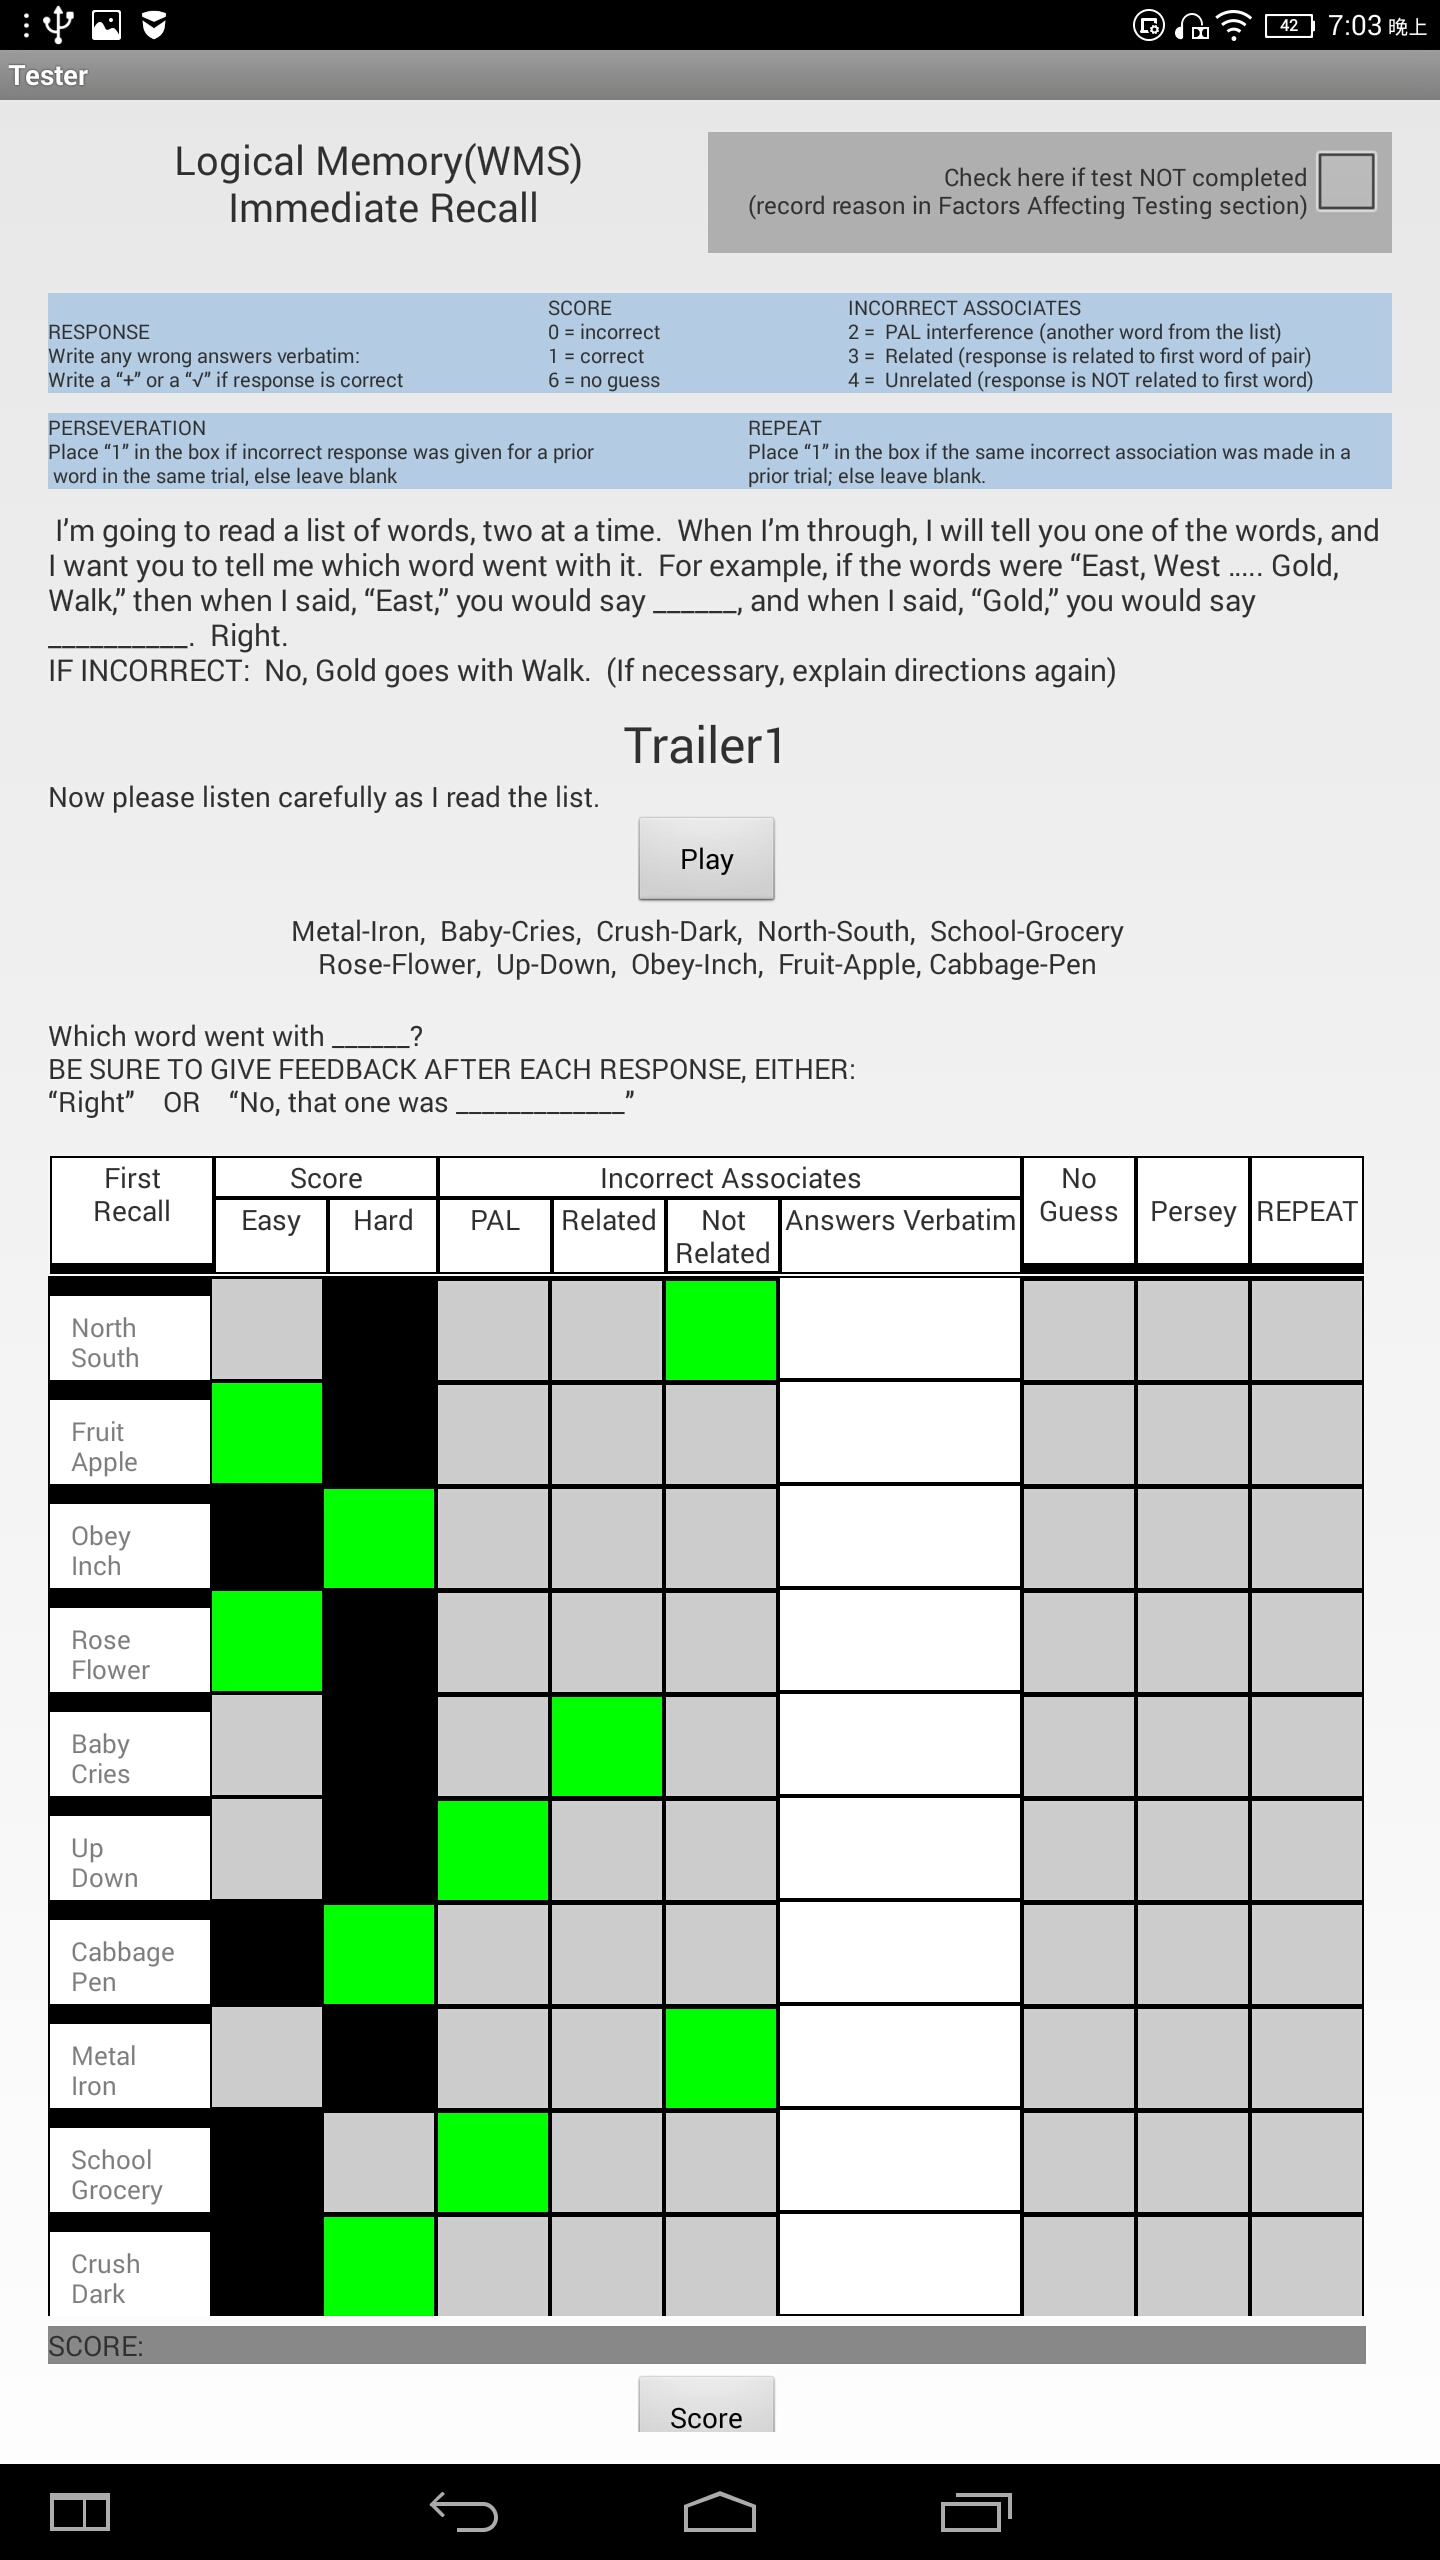
\includegraphics[width=6cm]{trailer}
\caption{单词对复述题-最终实现}
\end{subfigure}
\caption{单词对复述题设计和最终实现图}
\label{fig:big1-subfigure}
\end{figure}

单词对复述题模块的在线测试版和离线打分版一样。这个模块略微复杂,为整个模块设计了对应的界面组件:TrailView和SingleTrailView。其中SingleTrailView只包含一个单词对,而TrailView包含的是一组单词对(TrailActivity包含若干个TrailView,每个TrailView包含若干个SingleTrailView)。一个SingleTrailView包含了一个单词对和其对应的题目显示(包括多个按钮、输入框);TrailView除了包含多个SingleTrailView外还包含一些题目其他信息和获取分数按钮。这样设计是因为每个单词对是相互独立的,SingleTrailView让他们的按钮都能关联起来,TrailView不用管每个单词对的内部逻辑,让结构更简单化。在逻辑中,当Activity启动时,将题目内容更新到其成员TrailView,再让该成员将对应内容更新到TrailView。当用户对题目进行回答时,修改的是SingleTrailView,这时在SingleTrailView中会临时存储用户的答案。获取分数的按钮被设置在TrailView中,当用户点击时会TrailView会从成员SingleTrailView获取到答案信息并更新(但不会告知Activity)。只有当用户在界面上点击“下一页”时,才会从TrailView获取到答案并更新(当然,TrailView会递归地从SingleTrailView获取答案)和上传。

这里为了方便用户的一些操作,设计了“错误字典”,即每个错误的单词会记录下它的错误类型,这样在之后的输入中只要错误单词在字典中,就能很快得得到它的错误类型而不需要再进行错误类型的选择。

单词对复述题分为两种,一种是即时回答,另一种是稍微回答,界面略有不同,模块会根据题目JSON中的信息进行区分并展现不同的界面。


\section{数字串复述题模块}

\begin{figure}[h]
\centering%
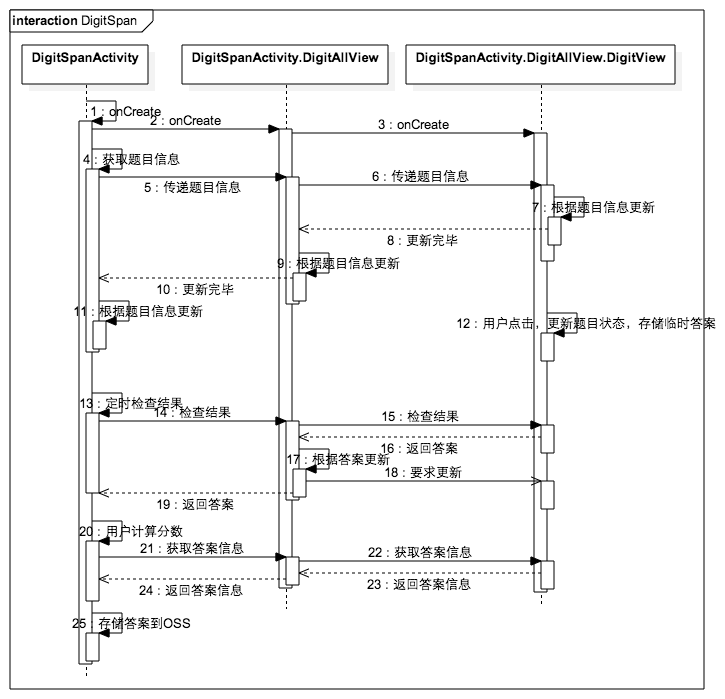
\includegraphics[width=13cm]{DigitSpan}
\caption{数字串复述题逻辑流程图}
\label{fig:big1-subfigure}
\end{figure}

\begin{figure}[h]
\centering%
\begin{subfigure}{6cm}
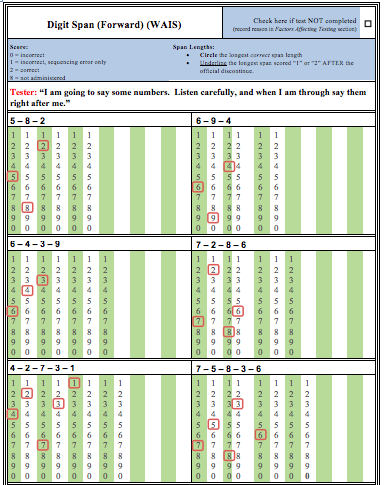
\includegraphics[width=6cm]{digitD}
\caption{数字串复述题-设计}
\end{subfigure}
\hspace{4em}%
\begin{subfigure}{6cm}
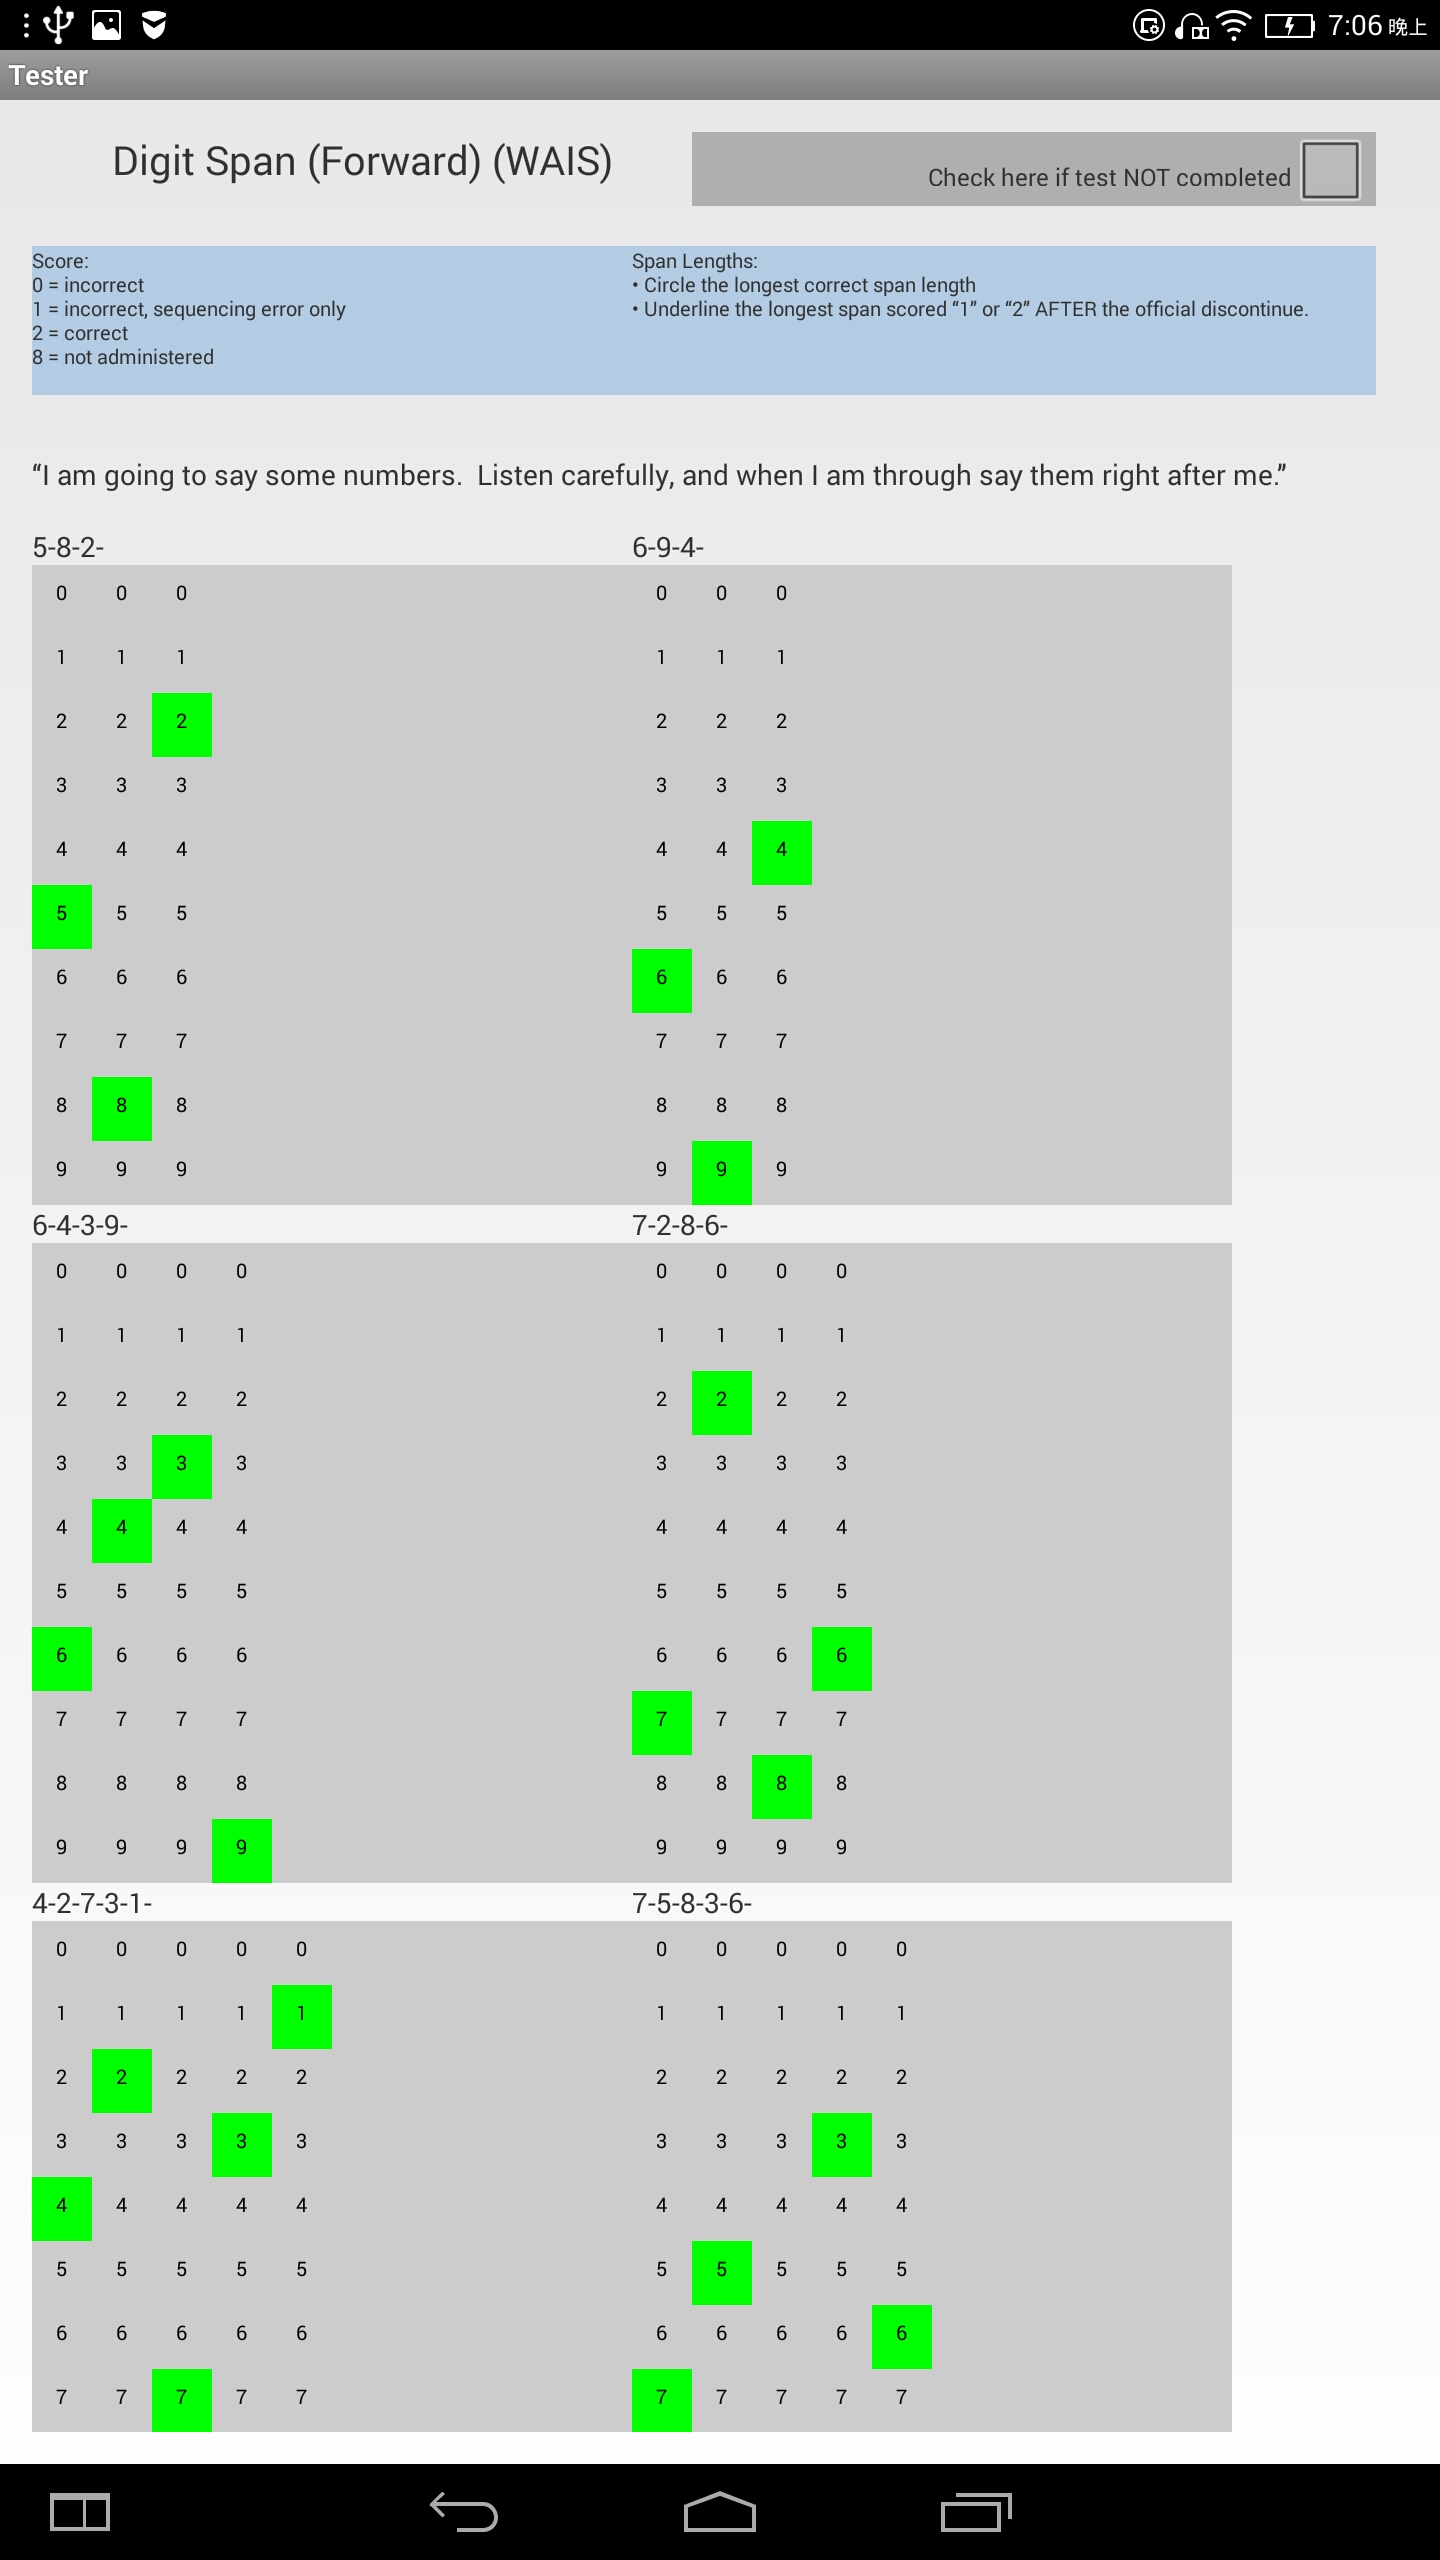
\includegraphics[width=6cm]{digit}
\caption{数字串复述题-最终实现}
\end{subfigure}
\caption{数字串复述题设计和最终实现图}
\label{fig:big1-subfigure}
\end{figure}

数字串复述题模块也相对复杂,与单词对复述题类似,设计了对应的界面组件:DigitAllView和DigitView。DigitView包含了一列可选数字(0-9),而DigitAllView是包含了一道数字串复述的题目。这样的设计思想和单词对复述题的设计思想类似,将独立的部分分开,使系统结构更简单更清晰。当Activity启动时会依次更新DigitAllView和DigitView。DigitView负责实时根据用户的选择更新答案。当用户需要计算分数,或是存储答案,则依次从两个组件中获取答案并更新、上传。

为了做到引导医生使用,模块设计也按照顺序显示题目,即开始只显示第一题,第一题结束后根据结果显示下一题。故在Activity中设置了Handler,以200毫秒更新的频率检查所有的DigitAllView,如果满足条件,则让其开启下一题。

\section{选择题模块}

\begin{figure}[h]
\centering%
\begin{subfigure}{6cm}
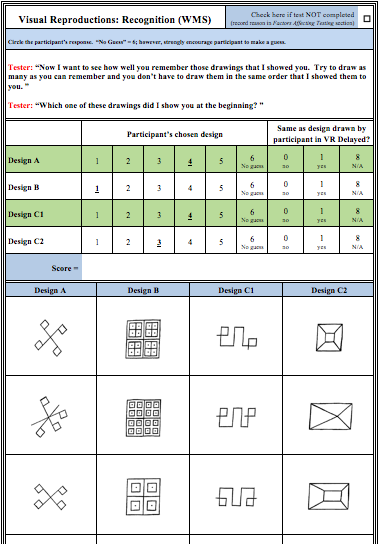
\includegraphics[width=6cm]{choiceD}
\caption{选择题-设计}
\end{subfigure}
\hspace{4em}%
\begin{subfigure}{6cm}
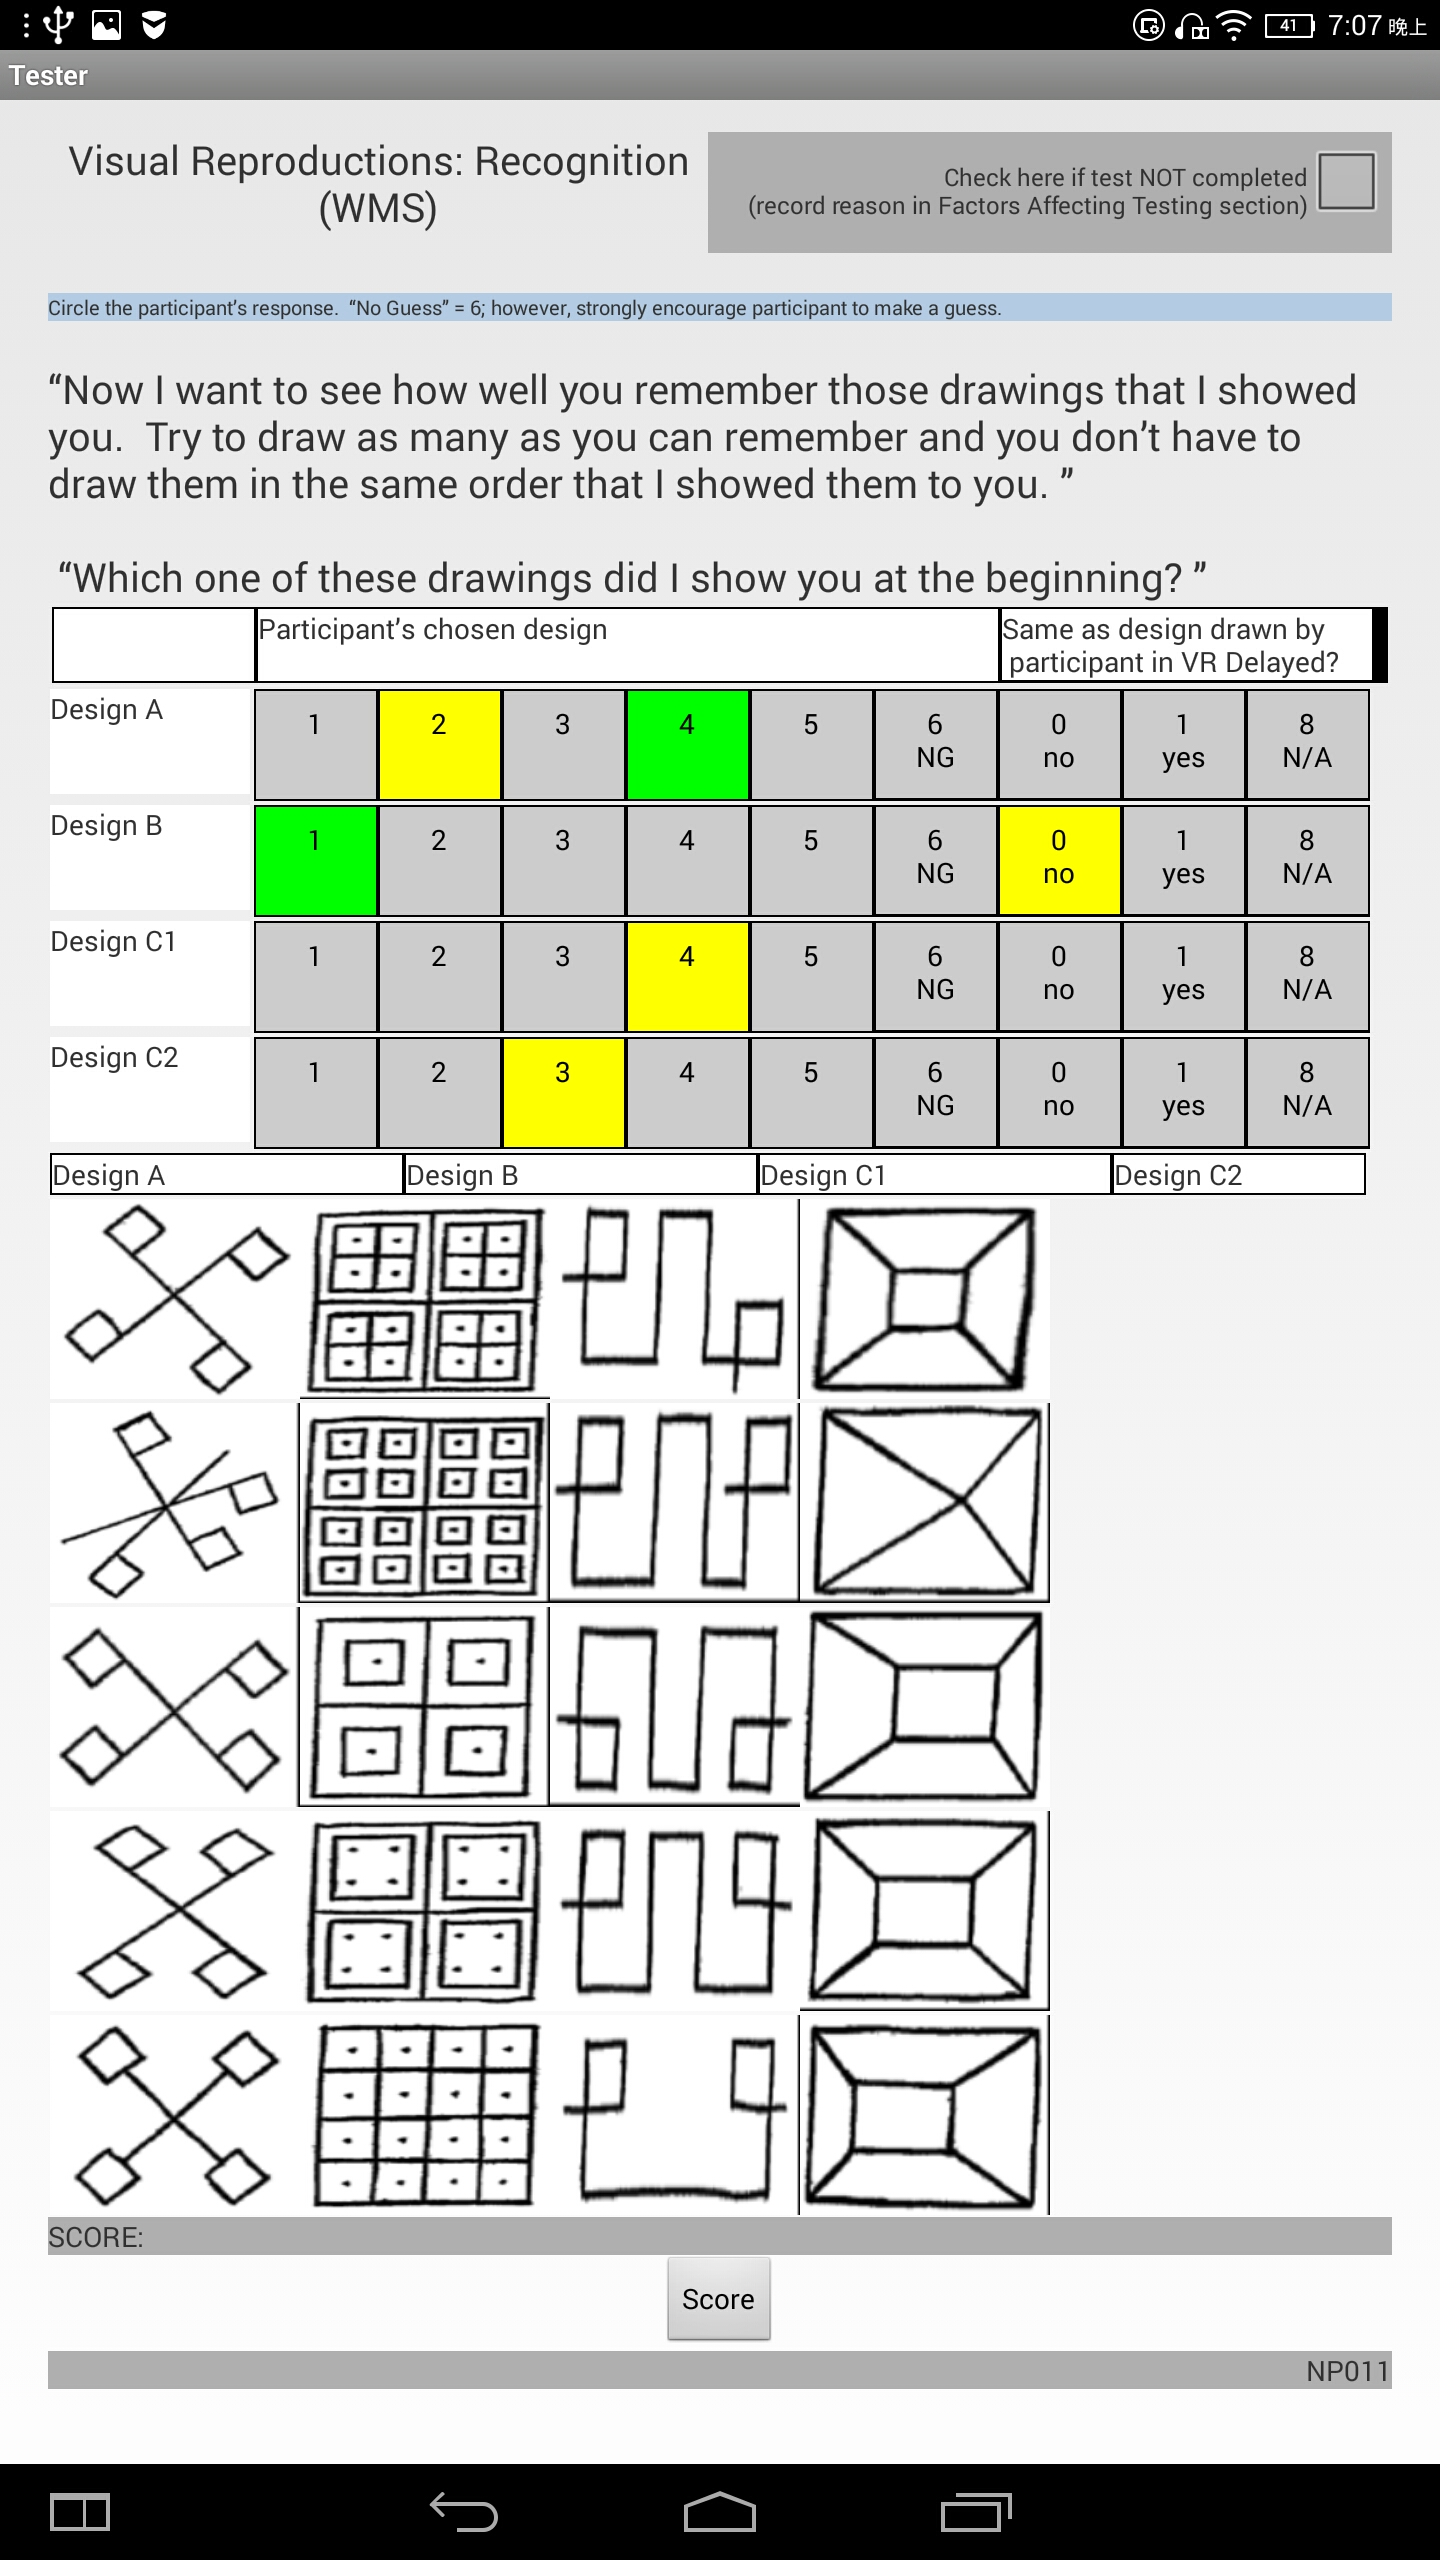
\includegraphics[width=6cm]{choice}
\caption{选择题-最终实现}
\end{subfigure}
\caption{选择题设计和最终实现图}
\label{fig:big1-subfigure}
\end{figure}

为了应对选择题有不同选项、不同表头要求,同样按照数字串复述题和单词对复述题设计了对应界面组件ChoicerView来表示一个选题和其关联的各选项,并临时存储用户选择的答案。当用户需要获取分数时,从每个ChoicerView获取答案并进行统计。当用户需要上传结果时,也从ChoicerView中获取答案并存储。

由于选择题有一种选择画图题,需要另建新图片选择表,在这里直接实现在了Activity里根据对应位置设置了图片按钮,并与对应题目进行关联。临时答案依旧存储在ChoicerView中。


\section{其他模块}

目前设计的其他模块只有结束界面,因为不需要花俏的界面,目前只有显示一行“Finished. Thank you!”的字样。




%%% Local Variables: 
%%% mode: latex
%%% TeX-master: t
%%% End: 

\chapter{测试}

\section{测试方法}

对Android系统的测试主要包括用户体验测试、业务测试、系统测试、功能模块测试、异常测试等等。由于本系统内没有大部分需要CPU性能的部分、并且本系统已经确定了硬件设备,工程编写和测试也变得比较简单:除了单元测试,使用、模拟测试(即在真机上运行程序对各项功能、界面等进行测试)是主要的测试方法。为了方便检查出错问题,在工程中多处加入了日志的输出,以便确认正确和出错的地方。主要通过运行程序对系统的各功能(界面展示、数据记录、逻辑处理等)进行了确认,以及对断网、多个用户访问、中断退出,并模仿一些恶意行为进行了测试。

最后,在多台对程序顺利安装、卸载、界面信息是否正确进行了测试。

\section{测试结果}

除了自己测试之外,我们也邀请了波士顿大学的学生测试使用该系统。测试反馈功能、界面以及数据系统均表现正常、没有异常发生。

由于时间的限制,目前只进行了一些初步的模拟测试,波士顿大学的学生会进行更深入的测试,并且已经安排了学生,继续改进。




%%% Local Variables: 
%%% mode: latex
%%% TeX-master: t
%%% End: 

\chapter{总结}

本文主要基于认知功能障碍传统的长问卷制作了辅助诊断的一整个系统,实现了画图题、录音题、选择题等多种题型。该系统建立在Android操作系统上,具有记录轨迹、录制和播放音频、逻辑判分等功能,也拥有独立和统一的数据系统。该系统也具有比较好的复用性和拓展性。

通过本次毕业设计,基于一个拥有多题型的问卷,根据其需求设计了一个能够方便自定义、结构和数据统一化的系统,并按照设计实现了三个版本的APP。在这个过程中,经历了一系列相关领域、功能的调研,试用了一些现有的服务、进行了实验来验证性能并选择了使用的服务;然后经过参考多个系统的结构,设计了一整套可用、统一的系统,并对自己的设计进行了实现,最后在选择的硬件上安装APP进行了测试,并得到了合作方的确认。

在本次毕业设计中,我的主要贡献在提出了基于三个版本(在线医生版、在线病人版和离线打分版)、数据和结构统一化的系统设计,其将各功能分开的特点具有编码简单、能够自定义各类题目以及扩展性和复用性强的好处;规定了题目和答案的存储方案,具有扩展性强、自由性强、安全性强、找回率高的特点;另外也根据题目的需求设计了各题的展示界面,不仅复原了纸版问卷的题目,同时具有方便易用、也易学会的特点。


%%% 其它部分
\backmatter

% 本科生要这几个索引,研究生不要。选择性留下。
\makeatletter
\ifthu@bachelor
  % 插图索引
  \listoffigures
  % 表格索引
  \listoftables
  % 公式索引
  %\listofequations
\fi
\makeatother


% 参考文献
%\bibliographystyle{thubib}
%%% Local Variables: 
%%% mode: latex
%%% TeX-master: "../main"
%%% End: 

\begin{center}
\chapter*{参考文献}
\end{center}

\begin{enumerate}[{$[$}1{$]$}]
\item John E Harrison, Angela Caveney. 10 Years of the Neuropsychological Test Battery.
\item 李焰生《中国防治认知功能障碍专家共识》,中华老年医学杂志2006年7月第25卷第7期
\item X Ducrohet, T Norbye, K Chou. Android Studio: An IDE built for Android.
\item BC Zapata. Android Studio Application Development.
\item W Chigona, M Nyemba, A Metfula. A review on mHealth research in developing countries. 2012 The Journal of Community
\item E Alepis, C Lambrinidis, M-health: supporting automated diagnosis and electronic health records. 2013 Springer
\item R Wei, Z Yang. Design and Implementation of Doctor-Patient Interaction System Based on Android. 2012 Technology in Medicine and Education
\item C Benedict, SJ Brooks, J Kullberg, R Nordenskjöld. Association between physical activity and brain health in older adults. 2013
\item AJ Simon, DM Devilbiss. Systems and methods for the physiological assessment of brain health and the remote quality control of EGG systems. 2012 US Patent App. 14/233,292
\item M Bacchiani, A Senior. Asynchronous, Online, GMM-free Training of a Context Dependent Acoustic Model for Speech Recognition. 2014 International Speech
\item Y Wu, TS Huang. Vision-Based Gesture Recognition: A Review. 1999 Besture-based communication in human-computer interaction
\end{enumerate}



% 致谢
%%% Local Variables:
%%% mode: latex
%%% TeX-master: "../main"
%%% End:

\begin{ack}
衷心感谢导师陶霖密教授对本人的精心指导,感谢老师细心解答我在整个毕设过程中提出的一些繁琐的问题,也感谢老师愿意花大量时间在设计系统上提供指导、帮助和支持。感谢波士顿大学为这个系统提供的资料、测试和建议。感谢实验室学长张美庆同学在一些实现代码上的解答,感谢赵汉卿同学在轨迹识别模块的讨论与实验。

感谢刘佳倩同学提供了网络连接VPN,使得设计过程中工具和文献资料的下载更为顺利。感谢 \thuthesis,完美而迅速解决了论文的格式问题。

同时也感谢我身边的朋友、室友和同学们,毕设过程中因为有你们的相伴而不再枯燥,因为看到你们的努力而让我更加勤奋,因为你们的建议让我对专业有了更深的理解。

\end{ack}


% 附录
\begin{appendix}
%%% Local Variables: 
%%% mode: latex
%%% TeX-master: "../main"
%%% End: 

\chapter{书面翻译}
\begin{center}
\section*{基于安卓平台设计和实现的医患交互系统$^{[1]}$}
\end{center}

摘要-医疗服务的信息化已经成为了国际发展的一个趋势。随着信息技术的迅速发展,越来越多的医院为了改善医疗服务而加速了基于信息平台的整体服务的实现。移动互联网的发展为医药产业提供了全新的服务模式和发展方向。安卓是一个基于Linux平台开源的移动手机操作系统。因为它的开放性和便捷的开发方式,它在移动互联网的领域上有很高的地位。在这篇文章中,我们展现了一个基于安卓的医患交互系统。它在移动终端上出色的表现让病人能通过连接医院的服务器获取到关于病症建设性的意见,他们也可以通过这个交互系统和医生进行交流,同时医生们也可以在任何时刻、任何地点通过呈现在这些硬件移动终端上的数据跟踪病人的情况从而作出及时的诊断。

关键词:安卓;移动健康;移动互联网;移动定位


\section*{1. 介绍}

医患交互系统的建立和发展对于现在的医疗服务信息化来说是相当重要的需求,尤其是移动交流技术飞速发展的今天,移动互联网的诸多有点都能购被充分利用在弥补医生和病人之间时间和地理位置的差别从而提供快速、充足的医药服务,从而它已经成为了衡量一个医院是否有竞争力的重要指标。通过移动终端和专业服务的连接,医生和病人都能通过比传统更好的交互方式获取到数据。安卓是一个基于Linux平台的开源操作系统,它主要用于移动设备,它良好的性能使它的使用市场不断扩大。同时,网络应用和数据库技术这两个平台也正在逐渐地成熟,因此借助这些平台我们可以在安卓上开发一个医患交互系统去满足医生能更便捷和方便地治疗病人、和病人沟通的需求$^{[2]}$。

\section*{2. 安卓和移动健康}

HIMSS(医疗信息和管理系统安全)给出过关于移动健康的确切定义:即通过移动交互技术比如平板,手机和卫星系统来提供医疗服务或信息。随着现代移动技术的迅速发展,移动健康的规模和服务质量都在提升。为了开发一套方便的医患交互系统,使用成熟的集成终端平台已经变成了刚需。安卓的诞生给我们提供了很多便捷。

\subsection*{2.1 关于安卓}

安卓由操作系统、中间件、用户界面和应用软件组成$^{[3]}$。它开源的特性使得这个平台能够更快地发展新技术、有新创新,也让我们能够很容易地定制个性服务。在安卓上开发一个医患交互系统因为其市场地开放性能够有很好地商业前景、也能够很大程度上增加服务的竞争性。

\begin{figure}[h]
  \centering
  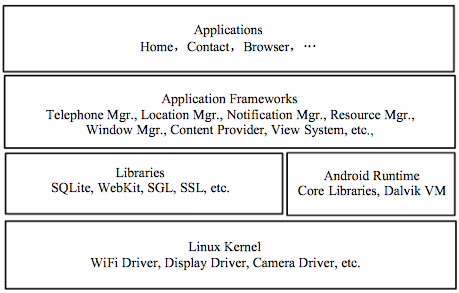
\includegraphics[clip]{paper-1}
  \caption*{图~1\hskip1em 安卓系统结构}
\end{figure}

\subsection*{2.2 关于移动健康}

近几年,移动健康成为了电子健康(指的是用信息交流技术如电脑,手机和卫星提供医药服务和信息)领域的重要分支。随着低成本的移动手机和全球流行化的移动互联网,成千上万曾经购买不起固定电话或电脑网络的人现在能够将手机作为一种日常交流和数据传输的工具,这也为使用移动技术来支持医药服务打下了扎实的奠基。

随着移动交互技术的发展,越来越多的服务能够更正规、快速和廉价得传播。网络带宽的变大、覆盖面的变广给为移动健康开发更好、更合适的应用提供了好的基础。

\section*{3. 系统设计}

我们提出的系统包括两个类型:医生用户和病人用户,这个系统也包括以下这些特征:症状和处方的查询,医患间非实时的通讯,病人地理位置,病人信息的监控。

\subsection*{3.1 症状和处方的查询}

在这里会运用一些缩写和简写。缩写不包括IEEE,SE,MKS,CGS,sc,dc和rms。在标题中会尽量不要使用缩写(除非不可避免)。

1) 原理分析:这个子模块是为了病人能够得到便捷的服务而设计的。一般得了小毛小病的病人能够通过这个服务访问医院的数据库以查看症状有关的信息和推荐的养生之道来达到自我检查的目的,这样可以节省病人和医生很多的时间和精力。

为了设计这个自模块我们需要同时考虑移动终端和用户行为的资源是有限的。首先,查询动作的周期应该越短越好,所以我们应该为用户提供很好的字典结构使得用户能够快速准确地获取查询地结果。其次,考虑到信息内容储存和表达应该达到最优的性能,移动终端应该以最快的速度根据性能的限制给用户展现查询结果。第三,移动终端应该能够直接支持HTML和XML以防止在信息传递的过程中用以查询结果的服务器返回的信息缺失一些内容导致整个原始内容的丢失。

2) 模块设计:首先我们需要在医院服务器上建立一个医药方法信息的数据库。临床疾病的分类、症状和治疗方案应该都需要存储在数据库平台里。关系数据库里应该为病人的查询包括主要器官的病理学、症状和治疗方案、建议的疗养方法的数据。

在移动终端设备上,我们用集成的数据库系统SQLite1.3来备份移动数据$^{[3]}$来保证系统在离线时也能整场运行。SQLite时一个开源的集成的数据库引擎。它能完全独立地提供几乎所有SQ192标准并且在所有主要地操作系统上运行。数据的一致性和扩展性应该通过同步移动端备份的数据和中央数据库而被保证的。这个系统使用SyncML协议在开源的funambol工程框架上做二阶开发$^{[4]}$。

\begin{figure}[h]
  \centering
  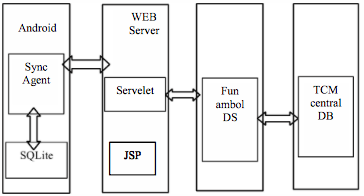
\includegraphics[clip]{paper-2}
  \caption*{图~2\hskip1em 数据同步自模块结构}
\end{figure}

\subsection*{3.2 医患间非实时通讯}

1) 原理分析:和医生的交流能够给病人更好的服务体验。即时通讯需要医生一直在线,然而这在医药界是不太合理的,所以非实时应该是医患交流的主要模式,也就是,病人能够在系统中留言或者提问,而医生也能够通过系统来回答这些问题。

目前的信息交换平台主要基于类似BBS的网页刷新机制,然而这样的传输方式的缺点在于数据量大,使得要消耗很多的流量,所以这不适合于移动终端的信息交流。非实时交流不仅强调信息的重要性,也强调回复操作能够方便和快速。因此最好的方式是结合互联网和常用的交流方式,比如传统新建。

2) 模块设计:在安卓平台上设计一个电子邮件系统需要系统直接支持POP3协议接受邮件、SMTP来发送邮件。这样可以解决传统手机靠短信传递信息的不方便和慢速,但前提是协议的回话以及用户在连续的网络环境里。移动医疗应该支持手机间的电子邮件通讯。这个电子邮件系统的框架可以见图3。

\begin{figure}[h]
  \centering
  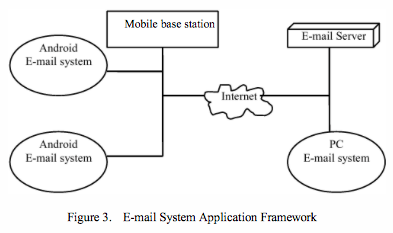
\includegraphics[clip]{paper-3}
  \caption*{图~3\hskip1em 邮件应用系统框架}
\end{figure}

\subsection*{3.3 病人地理位置}

1) 原理分析:通过移动终端获取地理位置对于医生和病人来说都是很重要的。比较严重的病患可以通过整体的GPS定位模块给医院发送他们的地理位置。当医院接受到病人的地理位置信息,就能够和服务器共享这个信息并找出离这个病人最近的服务,这样就节省了很多珍贵的时间。因此地理位置定位的模块也需要准确和快速。

2) 模块设计:在移动终端上开发一个GPS应用$^{[5]}$。在运行一个程序后,我们可以在它主界面之外开启一个新的线程而开启一个定期读取GPS数据从而获得当前用户位置信息,这样这些数据就能够存储在数据库里并且发送、分享给服务器。在安卓平台上GPS导航应用的开发已经相当成熟了,我们都可以通过注册认证自己的应用用Google地图的API接口获取Google地图的服务。

\begin{figure}[h]
  \centering
  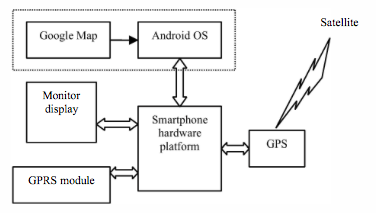
\includegraphics[clip]{paper-4}
  \caption*{图~4\hskip1em GPS导航系统的分析}
\end{figure}

\subsection*{3.4 病人信息的监控}

1) 原理分析:对于卧床的病人,医院需要监控他的各种信息,所以移动终端应该附有能够定时把病人病例信息传输到医院监控终端上以让医生能够诊断的能力。但这样的监控需要很多集成的通信模块和额外的医疗子模块。因为我们无法获取到所有硬件的需求,我们仅仅考虑常见的硬件资源:用相机的摄像头来获取视频监控功能,以提供最简单基础的监控信息。

2) 模块设计:这个模块包括视频收集模块、数据处理模块、图像展示模块。USB视频收集模块包括了USB摄像头、USB摄像头驱动两个模块。数据处理模块包括H.264解码库、收集和传输模块。整个工作流程可以参考图5。

\begin{figure}[h]
  \centering
  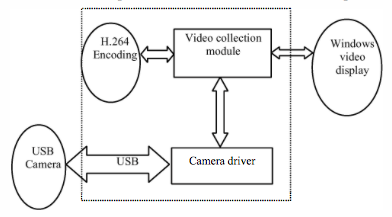
\includegraphics[clip]{paper-5}
  \caption*{图~5\hskip1em 监控系统的框架}
\end{figure}

\section*{4. 每个模块的关键部分}

\subsection*{4.1 病状和医疗方案模块中的数据获取}

1) 连接移动数据库:主要通过写程序调用移动数据库的接口来检查和组织病状和其医疗方案信息的特定分类。ListRecipe是这个系统中用来获取数据的一个子类$^{[6]}$,以下是一部分的接口代码:

\begin{lstlisting}[language=Java]
Cursor cur=getContentResolver().query(getlntent().getData(), PROJECTlON, sql, null, null);
\end{lstlisting}

2) 治疗方案的查询:通过安卓提供的元素接口,我们能够把界面展示和数据源结合来流畅展现对应的治疗方案、并且将模块安装到显示器上。ListRecipe也负责这一块,部分代码如下:

\begin{lstlisting}[language=Java]
SimpleAdapter adapter = new SimpleAdapter(this, fillMaps, R.layout.grid_item, from, to);
listView.setAdapter(adapter);
listView.setOnltemClickListener(this);
\end{lstlisting}

\subsection*{4.2 在医患非实时交流模块中的消息处理}

我们用来实现非实时通讯的基于安卓平台的移动端电子邮件主要包括的邮件发送和接收模块。系统需要处理文本或MIME(多目的电子邮件的拓展)的邮件类型。前者只包括两个部分:头(来自谁,发给谁,主题是什么)和主体(比如“你好X先生”之类)信息;而后者,信息被分成了若干个MIME分块,每个分块用一个特别的头信息来描述,比如常见的如表1,这样我们就需要对应的设置不同的类型。

\begin{table}[htbp]
\centering
\caption*{表A.1 不同类型}
\label{tab:ParametersForPandR}
\begin{tabular}[c]{lccc}
\toprule[1.5pt]
{\heiti 名称} & {\heiti 有效数值} & {\heiti 区分方法} \\\midrule[1pt]
MIME-版本 & 1.0 & MIME版本号 \\
内容-类型 & 文字,图片,语音,视频,应用,消息等 & 数据类型 \\
内容-传输-解码 & 7位或8位 & 数据解码类型 \\
\bottomrule[1.5pt]
\end{tabular}
\end{table}

\subsection*{4.3 病人地理位置信息模块的位置信息返回和分享}

我们通过编译继承于BroadcastReceiver的SMS\_Receiver类来完成位置定位需求信息的展示。在onReceiver函数中,先判断从监听的目的地是否是android.provider.Telephony.SMS\_RECEIVED$^{[6]}$。如果是,Bundle包的目的地会创建一个SMSMessage的数组。通过createFromPdu()函数以及SMS消息获取信息,然后通过getDisplayOriginationAddress()函数和getdisplayMessageBody()函数得到源码和信息内容如果信息包含LOCATION\_SMS,则通过以下两句代码开启位置服务:

\begin{lstlisting}[language=Java]
LocationManager mLocationManager = (Location_Manager)content.getSystemService(Context.LOCATION_SERVICE);
Location mLocation = getLocationProvider(mLocation_Manager);
\end{lstlisting}

然后经纬度的信息会通过一个SMS消息返回到移动收集用户,如果信息内容包含“LOCAL”,经纬度的信息会通过调用refreshMapView()函数来获取。

\subsection*{4.4 病人信息监控的视频收集}

在这个模块中我们使用数据报套接字(SOCK\_DGRAM)来达到视频数据的传递,因为这种方法在执行时比流套接字(SOCK\_STREAM)更快、成本更低。首先调用函数open("/dev/video0", 0\_RDWR)以打开视频设备。然后通过函数ioctl(fd, VIDIOCGCAP, \&rid\_cap)来获取类型video\_capability以读取摄像头图片的高度、宽度和其他相关信息。用mmap()内存匹配来获取视频图片。

\section*{5 总结}

在这里我们介绍了移动健康和安卓平台,设计了一套基于安卓的医患交互系统。在文章中我们分析了系统的应用需求和技术需求,并提升到了软件的层面,我们给出了基于有限硬件资源移动终端的医患交互模块主要部分的设计,并且确保了这些模块在安卓平台上是比较容易开发的$^{[8]}$。然而,系统依旧有一些缺点,比如如果物体在摄像头中变化比较大,展示模块的数据就会比较快的增长使得系统效率会降低。但由于安卓对于第三方应用的完全开放性,我相信未来会出现更好的服务,也会让移动健康这个领域有更好的性能。

\begin{center}
\section*{参考文献}
\end{center}

\begin{enumerate}[{$[$}1{$]$}]
\item R Wei, Z Yang. Design and implementation of doctor-patient interaction system based on android, ITME, 2012
\item Mark L.Murphy. The Busy Coder's Guide to Android Development. United States of America, Commons Ware, LLC., 2008
\item Justin\_luhui.baike.Baidu[EB/OL].[2010-10-12].
\item CHENG Chun-Iei, PAN Ze-qiang, "Research of chinese traditional medicine embeded information system based on android platform," Manufacturing Automation. pp 136-138. January 2011.
\item Shuiping Wei, Bangyan Ye, Zhiguang Fu, "Research on GPS Positioning Information Transfer Based on Wireless Network," 2007,28(6): 589-592.
\item Owens M., "Query Anything with SQLite," The World of Software Development, 2007, 32(12):24-28.
\item Jianxun Zhao, "Mobile Location Services Development and Implementation Based on Android Platform," Modern Business Trade Industry. pp 271-272. October 2010.
\item Chao-Tung Yang, Yen-Yu Chu, "Implementation of a Medical Information Service on Android Mobile Devices," New Trends in Information Science and Sercice Science, 2010(4):72-77.
\end{enumerate}

\begin{center}
\section*{书面翻译对应的原文索引}
\end{center}

\begin{enumerate}[{$[$}1{$]$}]
\item R Wei, Z Yang. Design and implementation of doctor-patient interaction system based on android, ITME, 2012
\end{enumerate}
\end{appendix}

% 个人简历
%\begin{resume}

  \resumeitem{个人简历}

  xxxx 年 xx 月 xx 日出生于 xx 省 xx 县。
  
  xxxx 年 9 月考入 xx 大学 xx 系 xx 专业,xxxx 年 7 月本科毕业并获得 xx 学士学位。
  
  xxxx 年 9 月免试进入 xx 大学 xx 系攻读 xx 学位至今。

  \resumeitem{发表的学术论文} % 发表的和录用的合在一起

  \begin{enumerate}[{[}1{]}]
  \item Yang Y, Ren T L, Zhang L T, et al. Miniature microphone with silicon-
    based ferroelectric thin films. Integrated Ferroelectrics, 2003,
    52:229-235. (SCI 收录, 检索号:758FZ.)
  \item 杨轶, 张宁欣, 任天令, 等. 硅基铁电微声学器件中薄膜残余应力的研究. 中国机
    械工程, 2005, 16(14):1289-1291. (EI 收录, 检索号:0534931 2907.)
  \item 杨轶, 张宁欣, 任天令, 等. 集成铁电器件中的关键工艺研究. 仪器仪表学报,
    2003, 24(S4):192-193. (EI 源刊.)
  \item Yang Y, Ren T L, Zhu Y P, et al. PMUTs for handwriting recognition. In
    press. (已被 Integrated Ferroelectrics 录用. SCI 源刊.)
  \item Wu X M, Yang Y, Cai J, et al. Measurements of ferroelectric MEMS
    microphones. Integrated Ferroelectrics, 2005, 69:417-429. (SCI 收录, 检索号
    :896KM.)
  \item 贾泽, 杨轶, 陈兢, 等. 用于压电和电容微麦克风的体硅腐蚀相关研究. 压电与声
    光, 2006, 28(1):117-119. (EI 收录, 检索号:06129773469.)
  \item 伍晓明, 杨轶, 张宁欣, 等. 基于MEMS技术的集成铁电硅微麦克风. 中国集成电路, 
    2003, 53:59-61.
  \end{enumerate}

  \resumeitem{研究成果} % 有就写,没有就删除
  \begin{enumerate}[{[}1{]}]
  \item 任天令, 杨轶, 朱一平, 等. 硅基铁电微声学传感器畴极化区域控制和电极连接的
    方法: 中国, CN1602118A. (中国专利公开号.)
  \item Ren T L, Yang Y, Zhu Y P, et al. Piezoelectric micro acoustic sensor
    based on ferroelectric materials: USA, No.11/215, 102. (美国发明专利申请号.)
  \end{enumerate}
\end{resume}

\end{document}
